\documentclass[12pt, a4paper]{article}
\usepackage{fontspec}
\defaultfontfeatures{Ligatures={TeX},Renderer=Basic} 
\setmainfont[Ligatures={TeX,Historic}]{Times New Roman}
\usepackage[russian, english]{babel}
\usepackage{amsmath}
\usepackage{graphicx}
\usepackage{caption}
\usepackage{subcaption}
\usepackage{array}
\usepackage{titlesec}
\usepackage{setspace}
\usepackage{fancybox,fancyhdr}
\usepackage{titlesec}
\usepackage{lastpage}
\usepackage{float}
\usepackage{etoolbox}
\usepackage[titles]{tocloft}
\usepackage[top=3.5cm,bottom=2.5cm,left=2.5cm,right=2.5cm,headheight=17pt,includehead,includefoot,heightrounded]{geometry} 
\usepackage{xeCJK}
\setCJKmainfont{SimSun}
\bibliographystyle{plain}
\counterwithin{figure}{section}

\newcommand{\anonsection}[1]{\section*{#1}\addcontentsline{toc}{section}{#1}}

\begin{document}
	\begin{titlepage}
		\begin{center}
			\LARGE{\textbf{Dalian University of Technology Undergraduate Capstone Project (Thesis)}}
			~~~
			\\
			~~~
			\\
			~~~
			\\
			~~~
			\\
			~~~
			\\
			\Large{\textbf{Influence of vortex generators in a turbulent boundary layer on local friction and transport}}
			~~~
			\\
			~~~
			\\
			~~~
			\\
			~~~
			\\
			\begin{verse}
			\begin{minipage}{0.3\textwidth}
				Department:\\  
				Major:\\
				Name:\\                 
				Student Number:\\                
				Supervisor:\\          
				Review Teacher:\\
				Completion Date:\\
			\end{minipage}
			\hfill
			\begin{minipage}{0.6\textwidth}
				\underline{\hspace{1cm}DUT-BSU Joint Institute\hspace{1.9cm}}\\   
				\underline{\hspace{1cm}Engineering Mechanics\hspace{2.15cm}}\\  
				\underline{\hspace{1cm}Dima Shevelev\hspace{3.85cm}}\\   
				\underline{\hspace{1cm}1922241\hspace{5.15cm}}\\
				\underline{\hspace{1cm}PhD. Ass. Prof. Andrei Chorny\hspace{0.5cm}}\\ 
				\underline{\hspace{1cm}Prof. Zhuravkov Michael\hspace{1.75cm}}\\
				\underline{\hspace{1cm}2023-04-20\hspace{4.55cm}}\\  
			\end{minipage}
			\end{verse}
			~~~
			\\
			~~~
			\\
			~~~
			\\
			~~~
			\\
			\Large{大连理工大学}
			~~~
			\\
			Dalian University of Technology
		\end{center}  
	\end{titlepage}
	\newpage
	\pagestyle{fancy}
	\fancyhead[R]{Capstone Thesis}
	\fancyhead[L]{Dalian University of Technology}
	\fancyfoot[C]{-\thepage-}
	\begin{center}
		\textbf{原创性声明}
	\end{center}

	本人郑重声明:本人所呈交的毕业设计(论文),是在指导老师的指导下独立进行研究所取得的成果。毕业设计(论文)中凡引用他人已经发表或未发表的成果、数据、观点等,均已明确注明出处。除文中已经注明引用的内容外,不包含任何其他个人或集体已经发表或撰写过的科研成果。对本文的研究成果做出重要贡献的个人和集体,均已在文中以明确方式标明。
	\\\\
	本声明的法律责任由本人承担。
	~~~
	\\
	~~~
	\\
	~~~
	\\
	作者签名:\hspace{110pt}日  期:\\                 
	(Signed by the author)\hspace{40pt}(Date)
	\newpage
	\begin{center}
		\textbf{关于使用授权的声明}
	\end{center}
	本人在指导老师指导下所完成的毕业设计(论文)及相关的资料(包括图纸、试验记录、原始数据、实物照片、图片、录音带、设计手稿等),知识产权归属大连理工大学。本人完全了解大连理工大学有关保存、使用毕业设计(论文)的规定,本人授权大连理工大学可以将本毕业设计(论文)的全部或部分内容编入有关数据库进行检索,可以采用任何复制手段保存和汇编本毕业设计(论文)。如果发表相关成果,一定征得指导教师同意,且第一署名单位为大连理工大学。本人离校后使用毕业毕业设计(论文)或与该论文直接相关的学术论文或成果时,第一署名单位仍然为大连理工大学。
	~~~
	\\
	~~~
	\\
	~~~
	\\
	论文作者签名:\hspace{110pt}日  期:\\               
	(Signed by the author)\hspace{70pt}(Date)\\
	指导老师签名:\hspace{110pt}日  期:\\                
	(Signed by the instructor)\hspace{50pt}(Date)
	\newpage
	\tableofcontents
	\newpage
	\anonsection{Abstract}
	Turbulent boundary layers develop on the surfaces of many engineering structures: from heat exchange devices, elements of air-jet engines to aircraft airframes, ship hulls and large building structures. They determine both frictional resistance and heat transfer. The vortex structure of these layers opens up the possibility of changing it by influencing the process of vortex formation.
	
	One of the ways to control and reduce energy losses in a turbulent boundary layer is to use active and passive turbulence control methods, for example, installing transverse ribs (vortex generators) on the surface or introducing a heat flux into the walls. A deeper understanding of the features of the turbulent boundary layer can help reduce energy costs and improve the efficiency of various technologies.
	
	Theoretical methods for modeling and studying transport phenomena in the boundary layer can conditionally be classified into exact, asymptotic, numerical, and approximate methods. Approximate and numerical methods are more often used for mathematical modeling of transport phenomena and determining the efficiency of ongoing processes in industrial devices.
	
	The modern development of turbulence as a science is not possible without the use of powerful computers that implement various models and make it possible to identify their strengths and weaknesses. It is the computational experiment that today is the source of the development of turbulence models, which, in turn, are the basis for the creation of new computational tools.
	
	The purpose of this work is to study the effect of a vortex generator installed along the entire length of the channel on local friction and transfer. The ANSYS Fluent package was used for calculations and for post-processing of the received CFD Post data. The method of modeling large eddies was used as a method.\\
	
	\textbf{Keywords:} vortex generator, boundary layer, turbulence, large eddy simulation, local friction and transport, grid model, modeling, analysis.\\	
	\newpage
	\section{Theory of boundary layer and it's modeling}
	\subsection{Concept of boundary layer}
	The motion of viscous environment is almost always associated with transfer phenomena in the boundary layer, where friction resistances, heat and mass transfer are localized. The concept of a boundary layer was first used by Ludwig Prandtl in an article presented on August 12, 1904, at the third International Congress of Mathematicians in Heidelberg, Germany. Boundary layer - the area of the flow of a viscous fluid with a small transverse thickness compared to the longitudinal dimensions, which is formed near the surface of a streamlined solid body or at the interface between two fluid flows with different velocities or temperatures. The boundary layer is characterized by a sharp change in the transverse direction of velocity (dynamic boundary layer) or temperature (temperature boundary layer).
	
	A classic example of a boundary layer is the boundary layer, which is formed on a thin plate when a liquid flows around its surface, and the boundary layer in round pipes. More difficult to study and mathematically describe is the boundary layer on surfaces with different curvature (flow around a cylinder, sphere, and other bodies). Such a boundary layer is characterized by a large pressure gradient and a separation point, beyond which the derivative and the flow velocity change signs. The boundary layers at the interface between two-phase and multi-phase environment are also much more complex.
	
	The lower the viscosity of the environment, the thinner the hydrodynamic boundary layer and the greater the significance of the velocity gradient in this layer. Outside the boundary layer, the velocity gradient is small. Consequently, the friction forces here are small and are usually neglected. There is no sharp boundary between the external flow and the boundary layer, since the average fluid velocity over the flow cross section changes monotonically, without jumps. Usually, the thickness of the boundary layer is determined conditionally, based on the fact that at its outer boundary the velocity is 99\% of the velocity of the external flow.
	
	\begin{figure}[H]
		\centering
		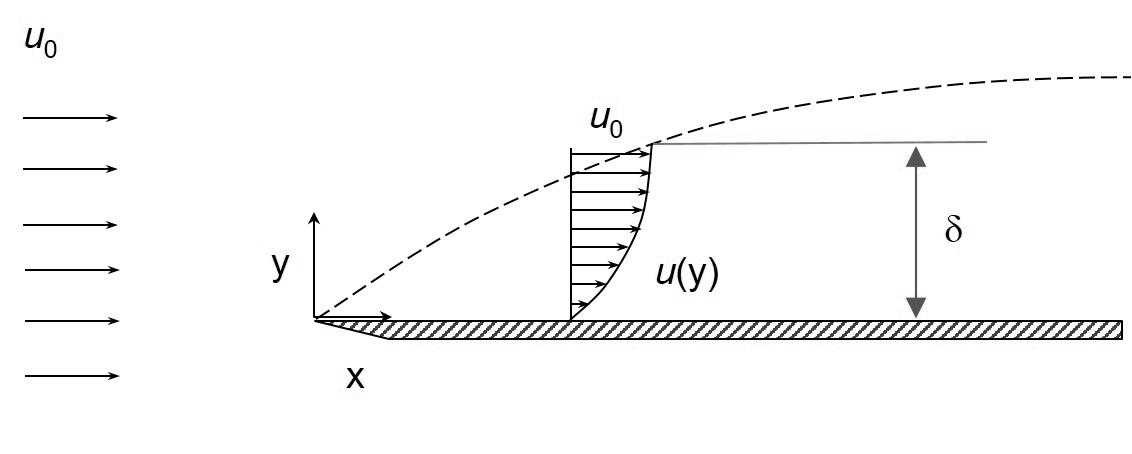
\includegraphics[width=0.7\linewidth]{../Assets/screenshot001}
		\caption{Boundary layer}
		\label{fig:screenshot001}
	\end{figure}
	The value of the boundary layer is very large, since it determines the hydrodynamic resistance when the environment moves relative to the solid body, as well as the resistance to mass and heat transfer. The introduction of this concept significantly simplified the equations for modeling the fluid flow by dividing the flow into two regions.
	
	In the general case, the non-isothermal motion of a viscous compressible fluid is described by the following equations: the Navier-Stokes equations, the equation of continuity, convective heat conduction and state.
	\begin{align}
		& u\frac{\partial u}{\partial x} + v\frac{\partial u}{\partial y} + w\frac{\partial u}{\partial z} = -\frac{1}{\rho}\frac{\partial p}{\partial x} + \nu(\frac{\partial^2 u}{\partial x^2} + \frac{\partial^2 u}{\partial y^2} + \frac{\partial^2 u}{\partial z^2}) \nonumber\\
		& u\frac{\partial v}{\partial x} + v\frac{\partial v}{\partial y} + w\frac{\partial v}{\partial z} = -\frac{1}{\rho}\frac{\partial p}{\partial y} + \nu(\frac{\partial^2 v}{\partial x^2} + \frac{\partial^2 v}{\partial y^2} + \frac{\partial^2 v}{\partial z^2})\nonumber\\
		& u\frac{\partial w}{\partial x} + v\frac{\partial w}{\partial y} + w\frac{\partial w}{\partial z} = -\frac{1}{\rho}\frac{\partial p}{\partial z} + \nu(\frac{\partial^2 w}{\partial x^2} + \frac{\partial^2 w}{\partial y^2} + \frac{\partial^2 w}{\partial z^2})\nonumber\\
		& \frac{\partial u}{\partial x} + \frac{\partial v}{\partial y} + \frac{\partial w}{\partial z} = 0 \nonumber\\
		& \rho c (\frac{\partial T}{\partial\tau} + \vec{v}\nabla T) = div(\lambda grad(T)) + q_v + \mu\Phi - p div(\vec{v}) \nonumber\\
		& f(p, \rho, T) = 0
	\end{align}
	Based on this, we have 6 equations and 6 unknowns ($u, v, w, \rho, T, p$). This system is extremely complex and, in general terms, is difficult to solve even by modern numerical methods on powerful computers. Therefore, various simplifications of this system are often considered.
	
	There are three types of flow in the boundary layer, each of which has its own characteristics and some of them are quite complex for numerical simulation:
	\begin{itemize}
		\item laminar -- the movement of the fluid is ordered, the layers do not mix, the particles rotate within the same thin layer;
		\item turbulent -- the motion is disordered, particles are mixed in the transverse direction and the entire boundary layer is randomly swirling;
		\item mixed -- transitional state from laminar to turbulent motion.
	\end{itemize}
	In this paper, we study the turbulent flow regime. It is more difficult for numerical simulation.
	
\subsection{Turbulent state of the boundary layer}
	The laminar flow is stable only under certain conditions determined by the value of the critical Reynolds number $Re_{cr}$. Usually, the transition from laminar to turbulent fluid flow in pipes is observed at $Re_{cr} \approx 2300$. Turbulent motion in the boundary layer arises from flow instability, which manifests itself in the form of vortices of various sizes and intensities. These vortices mix the liquid layers, which leads to an increase in the transfer of mass and energy along the surface of the solid. A turbulent flow with a large Reynolds number is called developed turbulence.
	
	The value of the critical number can be influenced. If the pipe inlet is made smooth, then laminar motion in the pipe can be appear at high Reynolds numbers, for example, up to 24000. $Re_{cr}$ is also significantly affected by such factors as pressure gradient, channel shape, roughness of its walls, injection and pumping of boundary layer. An increase in pressure in the direction of motion leads to instability of the flow in the boundary layer, separation, and the appearance of vortices. Therefore, both for internal (in pipes and channels) and external (flow around bodies) flows, the critical Reynolds number increases with a decrease in the external pressure gradient (accelerating flows - according to Bernoulli's law).
	
	\begin{figure}[H]
		\centering
		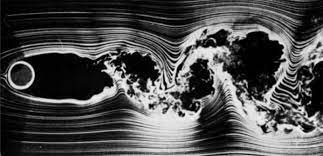
\includegraphics[width=0.7\linewidth]{../Assets/turb}
		\caption{Example of turbulence}
		\label{fig:turb}
	\end{figure}
	
	Turbulence can be defined as a three-dimensional unsteady motion in which, due to the stretching of vortices, a continuous distribution of velocity fluctuations is created in the range of wavelengths from the minimum, determined by viscous forces, to the maximum, determined by the boundary conditions of the flow. In the mathematical description of turbulent flows, it is convenient to proceed from the understanding of turbulence as a hierarchy of eddies of various scales, using the eddy and wave interpretation of turbulence\cite{Монин1992}. Turbulent eddies are continuous and constantly in contact with each other, and large eddies, the dimensions of which are determined by the boundary conditions of the problem, contain smaller eddies.
	
	The maximum size of vortices is close to the characteristic linear scale of the problem $L$. Often the motion of the largest vortices turns out to be largely ordered (for example, the flow behind a cylinder). Such structures are often called coherent. Vortices of the minimum size dissipate directly into heat. Their size is characterized by the Kolmogorov scale $(\nu^3/\epsilon)^{1/4}$. In this case, vortices of a certain average size carry the greatest amount of energy.
	
	One of the important characteristics describing turbulent motion is vorticity $\omega$: 
	\begin{align}
		\vec{\omega} = \vec{\nabla}\times \vec{v} \qquad \omega_x = \frac{\partial w}{\partial y} - \frac{\partial v}{\partial z}, \qquad \omega_y = \frac{\partial u}{\partial z} - \frac{\partial w}{\partial x}, \qquad \omega_z = \frac{\partial v}{\partial x} - \frac{\partial u}{\partial y}
	\end{align}

\subsection{Boundary layer structure}
	Ideas about the structure of the velocity profile gradually changed and were finally formed by the end of the 1950s. In a turbulent boundary layer, several regions are usually distinguished: external and internal. They differ from each other by different scales of vortex structures.\cite{Белов2001}.
	\begin{figure}[H]
		\centering
		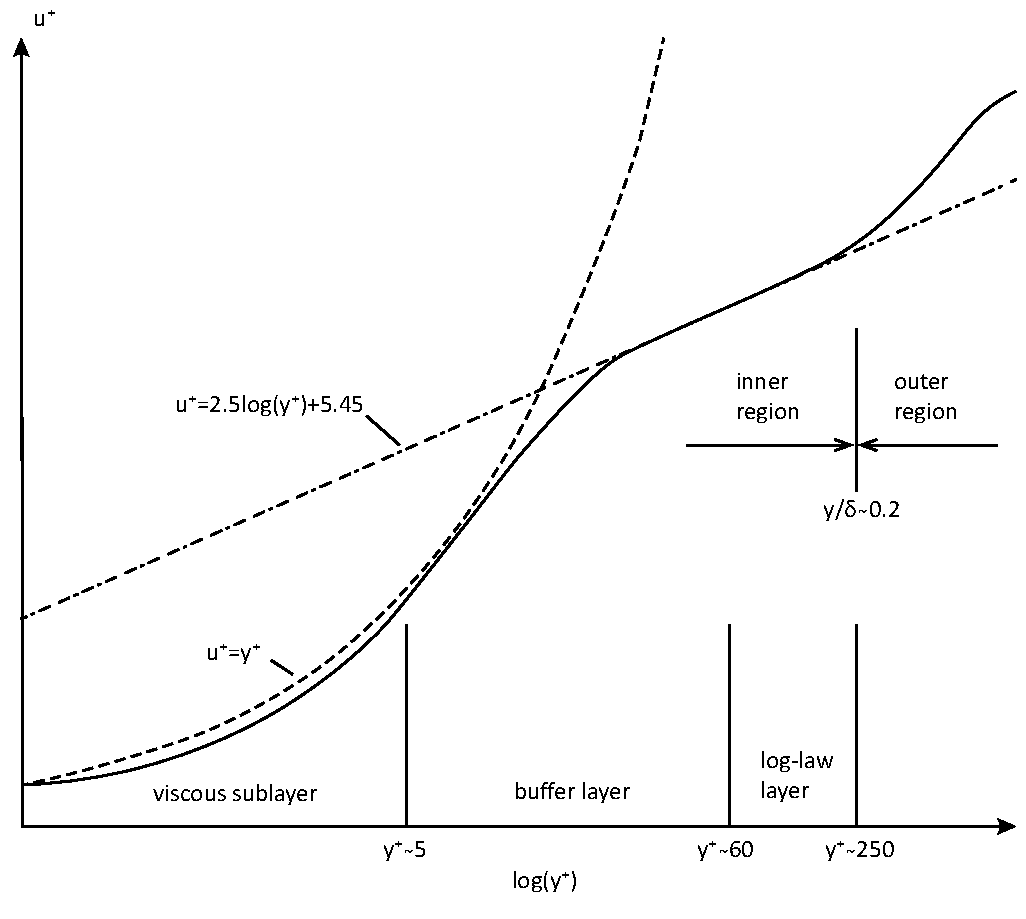
\includegraphics[width=0.7\linewidth]{../Assets/ПогранСлойEN}
		\caption{Layer structure}
	\end{figure}
	The inner region of the boundary layer occupies approximately 20\% of the thickness of the entire layer and generates up to 80\% of the turbulence energy in it. The formation of flow in the boundary layer is mainly influenced by the viscosity, thermal conductivity, and diffusion capacity of the liquid. Inside the dynamic boundary layer, there is a smooth change in velocity from its value in the external flow to zero on the wall due to the adhesion of a viscous fluid to a solid surface. Similarly, the temperature changes smoothly inside the boundary layer.

\subsubsection{Outer area}
	The outer layer is an area of fully developed turbulent flow, in which the velocity distribution is described by a logarithmic law. Complete damping of perturbations in the outer region occurs at a distance many times greater than the linear scale of turbulence.
	
	The filtered or Reynolds-averaged Navier-Stokes equations are used to determine the flux in the outer zone. At the same time, the velocity profile in the inner zone depends relatively little on various external conditions, such as Reynolds numbers and pressure gradient, which makes it possible to use universal relations (wall functions) to relate the flow parameters to the distance from the wall. This method is also based on the hypothesis of local equilibrium of the energy of turbulent fluctuations and the local isotropy properties of dissipating vortices

\subsubsection{Inner area}
	The viscous sublayer, buffer and logarithmic layers make up the inner region of the boundary layer. It is characterized by a high rate of mass, momentum and heat transfer, resulting in increased friction and energy loss.
	\begin{align}
		v\frac{\partial u}{\partial y} \gg -\overline{u'v'} & \qquad\text{viscous}\nonumber \\
		v\frac{\partial u}{\partial y} \approx -\overline{u'v'} & \qquad\text{buffer}\nonumber \\
		v\frac{\partial u}{\partial y} \ll -\overline{u'v'} & \qquad\text{log-law}
	\end{align}

	There are two approaches to modeling the flow in the near-wall region. In the first approach, semi-empirical formulas (wall functions) are used to describe the inner layer of the flow, while in the second approach, the turbulence models are modified in such a way as to resolve the entire near-wall region of the flow, including the viscous sublayer, provided that the required grid resolution in the boundary layer is provided. Such turbulence models can be used to calculate turbulent flows in the entire computational domain (including the near-wall flow region).
	
\subsubsection{Boundary layer properties}
	The thickness of the boundary layer is difficult to determine both in the calculation and in the experiment. The following concepts are used to define: displacement thickness $\delta^*$ and momentum loss thickness $\theta$.
	\begin{equation}
		\delta^* = \int_{0}^{\infty}(1 - \frac{u}{U_0})dy \qquad \theta = \delta^{**} = \int_{0}^{\infty} \frac{u}{U_0}(1 - \frac{u}{U_0})dy
	\end{equation}

	In addition, the dimensionless parameter is used $H$:
	\begin{equation}
		H = \frac{\delta^*}{\theta}
	\end{equation}

	The Reynolds number is characterized by two quantities($Re_x$ и $Re_\theta$): distance from bottom wall $x$ and thickness $\theta$.
	\begin{equation}
		Re_x = \frac{xU_0}{\nu} \qquad Re_\theta = \frac{\theta U_0}{\nu}
	\end{equation}

	Using the friction stress on the wall $\tau_w$ we can calculate the coefficient of friction $C_F$ and dynamic velocity $u_\tau$:
	\begin{equation}
		\tau_w = \nu\frac{\partial u}{\partial y}\bigg|_W \qquad C_F = \frac{\tau_w}{0.5\rho U_0^2} \qquad u_\tau = \sqrt{\frac{\tau_w}{\rho}}
	\end{equation}
	
	An equally important characteristic of the boundary layers is the longitudinal pressure gradient:
	\begin{equation}
		\frac{dp}{dx} = -\rho U_0 \frac{dU_0}{dx}
	\end{equation}
	
	Boundary layers are often affected by the following factors: surface curvature $\kappa$, liquid pumping and pumping speed, surface roughness $k_s^+$(height of hillocks).
	\begin{equation}
		\kappa = \frac{\delta^*}{R} \qquad \frac{V_W}{u_\tau}, \frac{V_W}{U_0} \qquad k_s^+ = \frac{k_s u_\tau}{\nu}
	\end{equation}

	An important property of the boundary layer is the fulfillment of the integral momentum equation. The converse is also true: if the momentum ratio is not high, then the flat boundary layer equation is also not true for the flow. This may be the influence of the aggregate: the three-dimension of the flow, its non-stationarity, the influence of the increase in flow, the change in pressure across the boundary layer, the influence of normal Reynolds surges, etc.
	\begin{equation}
		\frac{d\theta}{dx} + \frac{dU_0}{dx}\cdot\frac{2 + H}{U_0}\theta - \frac{C_f}{2} = 0
	\end{equation}
	
\subsection{Law of the wall}
	In order to work with the boundary layer, dimensionless quantities are usually used: $u^+$ and $y^+$:
	\begin{equation}
		u^+ = \frac{u}{u_\tau} \qquad y^+ = \frac{yu_\tau}{v}
	\end{equation}
	In the viscous sublayer, the viscous stresses are much higher than the Reynolds ones, and the velocity depends linearly on the distance to the wall. In the buffer layer, the stresses have the same order. In the logarithmic layer, the Reynolds stresses are much higher than the viscous stresses, and the velocity profile is described by a logarithmic law.
	\begin{align}
		&u^+ = y^+ & 0 \leq y^+ < 5 & \qquad\text{viscous} \nonumber\\
		&u^+ \neq y^+ & 5 \leq y^+ < 60 & \qquad\text{buffer} \nonumber\\
		&u^+ = \frac{1}{Ka}ln E y^+ & 60 \leq y^+ < 0.2\delta & \qquad\text{log-law}
	\end{align}
	In this case, the Karman number $Ka$ and the parameter $E$, which depends on the surface roughness, are determined on the basis of experimental data. 
	\begin{equation}
		Ka = \frac{1}{u}\sqrt{\frac{R_x^2 + R_y^2 + R_z^2}{3}}
	\end{equation}
	
	Law of the wall can be considered as a solution to the equations of motion in a turbulent boundary layer obtained using the Prandtl mixing path model. It is usually assumed that the wall law is satisfied for $30 < y^+ < 200$. The specific implementation of the approach depends on the chosen turbulence model and the difference scheme used. The functions included in the wall law need to be modified to accurately describe the effects associated with possible surface roughness. The wall law is difficult to adapt to the calculation of flows with complex geometry on unstructured grids.

\subsection{Modeling methods}
	Despite the intensive development of computer technology and the impressive progress achieved in recent years both in the field of constructing efficient numerical algorithms designed to solve problems of hydromechanics and heat and mass transfer, and in the development of related software (mesh generators, interactive data entry systems and systems for visualizing the results of calculations), the problem of numerical simulation of turbulence, as it has been for many previous decades, still remains one of the most complex and urgent problems of fluid mechanics. Unlike laminar flows of a single-phase medium (liquid), the calculation of which, thanks to the achievements noted above, has become largely a routine procedure, reliable prediction of the characteristics of complex turbulent flows, which are of the greatest practical interest, is still difficult.
	\begin{figure}[H]
		\centering
		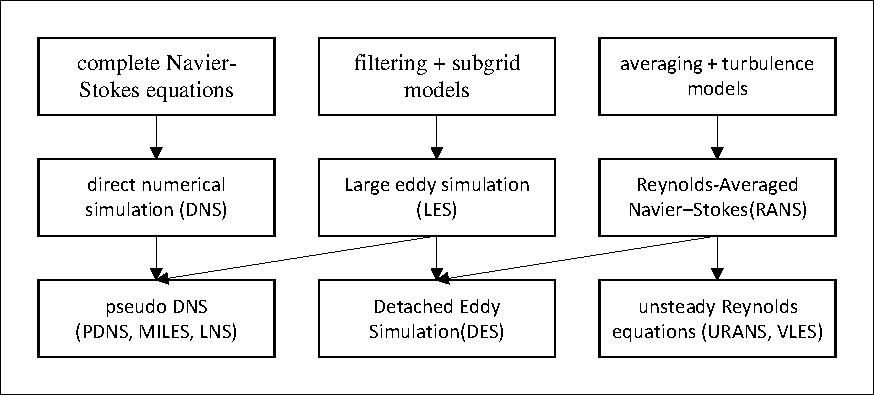
\includegraphics[width=0.9\linewidth]{../Assets/СхемаМетодовEN}
		\caption{Types of methods by equations}
		\label{fig:cheme}
	\end{figure}
	
	In computational modeling of turbulent flows, one common objective is to obtain a model that can predict quantities of interest, such as fluid velocity, for use in engineering designs of the system being modeled. For turbulent flows, the range of length scales and complexity of phenomena involved in turbulence make most modeling approaches prohibitively expensive; the resolution required to resolve all scales involved in turbulence is beyond what is computationally possible. The primary approach in such cases is to create numerical models to approximate unresolved phenomena. This section lists some commonly used computational models for turbulent flows.
	
	Turbulence models can be classified based on computational expense, which corresponds to the range of scales that are modeled versus resolved (the more turbulent scales that are resolved, the finer the resolution of the simulation, and therefore the higher the computational cost). If a majority or all of the turbulent scales are not modeled, the computational cost is very low, but the trade off comes in the form of decreased accuracy.
	
	In addition to the wide range of length and time scales and the associated computational cost, the governing equations of fluid dynamics contain a non-linear convection term and a non-linear and non-local pressure gradient term. These nonlinear equations must be solved numerically with the appropriate boundary and initial conditions.
	
	Among the main methods of numerical simulation of three-dimensional turbulent flows are: direct numerical simulation (DNS), simulation of large eddies (LES) and solution of Reynolds-averaged Navier-Stokes equations (RANS). There are also various intermediate approaches that combine certain features of RANS, LES, and DNS, for example, the detached eddy modeling method (DES), and a number of others that do not have a proper physical justification and, therefore, are not widely used.
	
\subsubsection{DNS}
	Direct numerical simulation (DNS) involves solving the complete non-stationary three-dimensional Navier-Stokes equations, which makes it possible to obtain instantaneous characteristics of a turbulent flow. Problems with the widespread use of the DNS are associated with high requirements for the difference scheme used, satisfaction of the initial and boundary conditions, as well as limited computing resources. In this case, the computational domain should be sufficiently extended to accommodate the largest scales of turbulence, and the time integration step should be of the order of the Kolmogorov scale.
	\begin{table}[H]
		\begin{center}
			\begin{tabular}{|c|c|c|c|c|}
				\hline
				Re & 6.6$\times10^3$ & 2.0$\times10^4$ & 1.0$\times10^5$ & 1.0$\times10^6$\\
				\hline
				Number of nodes & 2$\times10^6$ & 4$\times10^7$ & 3$\times10^8$ & 1.5$\times10^3$\\
				\hline
				150 MFlops & 37 h & 740 h & 6.5 years & 3000 years\\
				\hline
				1 TFlops & 20 s & 400 s & 8.3 h & 4000 h\\
				\hline
			\end{tabular}
		\end{center}
		\caption{Time spent for various parameters}
	\end{table}
	
	These stringent requirements are partly simplified by using high-precision spectral methods for the numerical integration of the Navier-Stokes equations, which are often used for DNS. However, these methods are not applicable to the calculation of flows with complex geometry. These circumstances lead to the fact that in practice the DNS is used only for calculating simple turbulent flows at low Reynolds numbers. In this case, the main task of the calculation is not actually obtaining data on the characteristics of the averaged flow (they are usually known), but obtaining detailed information about the structure of turbulence, as well as calculating individual terms included in certain turbulence models.
	
	However, direct numerical simulation is a useful tool in fundamental research in turbulence. Using DNS it is possible to perform "numerical experiments", and extract from them information difficult or impossible to obtain in the laboratory, allowing a better understanding of the physics of turbulence. Also, direct numerical simulations are useful in the development of turbulence models for practical applications, such as sub-grid scale models for large eddy simulation and models for methods that solve the Reynolds-averaged Navier–Stokes equations.
	
\subsubsection{RANS}
	Mathematical models based on the numerical solution of the Reynolds-averaged Navier-Stokes (RANS) equations are widely used in engineering applications. When using the Reynolds equations, the main interest is in the dynamics of large-scale eddies responsible for the transport properties of turbulent flows. When closing the Reynolds equations, we consider length scales typical of energy-containing vortices, in which $Re\gg1$ (except for near-wall areas). To take into account the near-wall influence of dissipating vortices and energy-containing vortices at $Re\sim1$ damping functions are used. Applying the Reynolds averaging to the equations, we obtain:
	\begin{align}
		&\frac{\partial u_i}{\partial x_i} = 0 \nonumber\\
		&\rho\frac{\partial u_i}{\partial t} + \rho u_j \frac{\partial u_i}{\partial x_j} = - \frac{\partial p}{\partial x_i} + \frac{\partial}{\partial x_j}(\mu\frac{\partial u_i}{\partial x_j} - \rho\overline{u_i' u_j'})
	\end{align}
	This system is not closed, since it includes an unknown tensor of the so-called Reynolds stresses $\tau_{ij} = -\rho\overline{u_i' u_j'}$(turbulent stresses). To close this system of equations, it is necessary to determine six different components of the symmetric turbulent stress tensor. It is the expression of these components in terms of the average flow parameters that is called the turbulence model. Below is a table with the main stages in the development of the theory.
	
	\begin{table}[H]
		\begin{center}
			\begin{tabular}{|c|c|c|}
				\hline
				Year & Scientist & Study\\
				\hline
				1877 & Boussinesq J. V. & Boussinesq conjecture\\
				\hline
				1895 & Reynolds O. & Reynolds averaging\\
				\hline
				1925 & Prandtl L. & Prandtl's mixing path theory\\
				\hline
				1930 & Theodore von Karman & Karman's formula\\
				\hline
				1942 & Kolmogorov A. N. & Kolmogorov formula, model $k$-$\omega$\\
				\hline
				1951 & Rotta & first Reynolds stress model\\
				\hline
				1956 & Clauser & Clauser formula\\
				\hline
				1956 & Driest E. R. & damping factor\\
				\hline
				1974 & Launder B. E.and Spalding D. B & model $k$-$\epsilon$\\
				\hline
			\end{tabular}
		\end{center}
		\caption{Stages of development of the theory}
	\end{table}
	
	The emergence of a huge number of models has led to the need of choice. To do this, it is necessary to conduct a comparative analysis of models. However, when trying to test in a natural way, certain difficulties arise. First, it is necessary to choose flows for which a set of reliable experimental data is known, free from errors, and also to choose criteria for comparing models. Secondly, it is necessary to carry out serial calculations of these flows using different turbulence models and, at the same time, be sure that the result is independent of the software implementation of the problem. The result of such work should be recommendations on the area of applicability of certain turbulence models.
	
\subsubsection{LES}
	The large eddy simulation method (LES) was proposed by Iosif Smagorinsky in 1963. It is based on two assumptions. The first assumes that the flow can be divided into the movement of large and small eddies. Large eddies that are under the direct influence of boundary conditions and carry the maximum of Reynolds stresses are calculated. Small-scale turbulence is considered to be isotropic and have universal characteristics, and therefore less critical and more amenable to modeling. Another is the possibility of approximating the nonlinear interactions between large and small eddies only by large eddies using subgrid models (SGS). In other words, the hypothesis of the statistical independence of large and small eddies is accepted.
	
	Large eddy statistics are usually insensitive to subgrid simulations, except for the near-wall region. Available subgrid models correctly predict not only averaged flow characteristics (first and second moments), but also fluctuations of integral characteristics, such as drag and lift coefficients\cite{Fureby2000}. Small-scale motion is eliminated from the Navier-Stokes equations by applying a filtering operation and modeled using subgrid models. On the image \ref{fig:lesfilter} the principle of operation of filters is shown, where $g(x)$ - original version, $f(x)$ - after filtration.\\
	\begin{figure}[H]
		\centering
		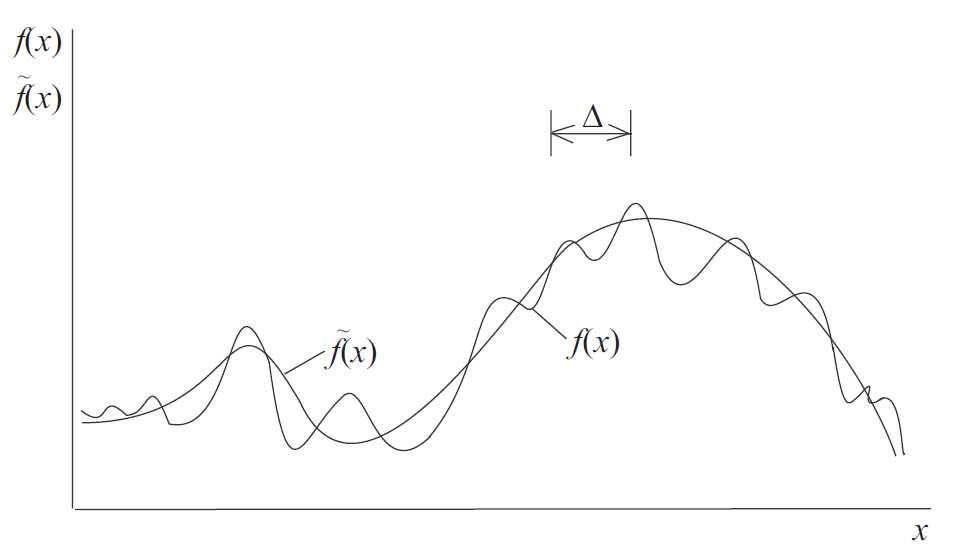
\includegraphics[width=0.7\linewidth]{../Assets/ФильтрацияLES}
		\caption{Exclusion of small-scale motions by filtering}
		\label{fig:lesfilter}
	\end{figure}

	Filter equation applied to the space-time field $\phi(x,t)$ presented below:
	\begin{equation}
		\overline{\phi(x,t)} = \int_{-\infty}^{\infty}\int_{-\infty}^{\infty}\phi(r,t')G(x - r, t - t')dt'dr
	\end{equation}
	In this case, $G$ is a kernel specific to each type of filter.
	
	The LES solution contains richer information than the Reynolds equation solution, for example, not only mean flow characteristics (velocity, concentration, temperature, pressure fields) and Reynolds stress distributions, but also spectral characteristics (pulsation spectra velocity and pressure), two-point moments, temporal and spatial scales of turbulence.
	
\subsubsection{DES}
	Large-scale unsteady three-dimensional vortex structures characteristic of separated flows are determined by specific boundary conditions and geometric characteristics of the flows under consideration and cannot be described within the framework of such models. This stimulates the search and development of hybrid approaches that combine the cost-effectiveness of RANS and the versatility of LES.
	
	In the detached eddy modeling (DES) method, in the region of the attached boundary layer, the method operates in the Reynolds equations mode, and in the region of flow separation it passes into LES. In this case, a combination of the best qualities of both approaches is achieved - the high accuracy and efficiency of the Reynolds equations in the region of the attached boundary layer and the universality of LES in the separation region. Although DES, unlike RANS, is a fundamentally non-stationary three-dimensional approach, the grids in the near-wall region required for its implementation coincide with the grids necessary for solving the Reynolds equations and are many orders of magnitude smaller than the grids required for resolving small near-wall vortices in the framework of LES. As the grid refines, DES asymptotically approaches LES and further to DNS. Specific implementations of DES are based on the use of the Spalart-Allmaras turbulent viscosity model and the Menter model\cite{Strelets2001}.
	
	As the name of the DES method implies, it was created to calculate separated flows. It is these currents that are best suited for this method. First, the presence of a massive separation in most cases leads to its pulsations, and as a consequence, to the emergence of a self-oscillating flow with large coherent structures. Secondly, the presence of a separation zone makes it possible to circumvent the problem of creating turbulent fluctuations at the entrance to the LES region.
	
\subsubsection{PDF}
	Probability density function(PDF) was introduced by Lundgren in 1969\cite{Lundgren1969}. This approach is analogous to the kinetic theory of gases, in which the macroscopic properties of a gas are described by a large number of particles. PDF methods are unique in that they can be applied in the framework of a number of different turbulence models; the main differences occur in the form of the PDF transport equation. For example, in the context of large eddy simulation, the PDF becomes the filtered PDF. In a more precise sense, the PDF is used to specify the probability of the random variable falling within a particular range of values, as opposed to taking on any one value. This probability is given by the integral of this variable's PDF over that range -- that is, it is given by the area under the density function but above the horizontal axis and between the lowest and greatest values of the range. The probability density function is nonnegative everywhere, and the area under the entire curve is equal to 1. The PDF is commonly tracked by using Lagrangian particle methods. When combined with large eddy simulation, this leads to a Langevin equation for subfilter particle evolution.
	\begin{figure}[H]
		\centering
		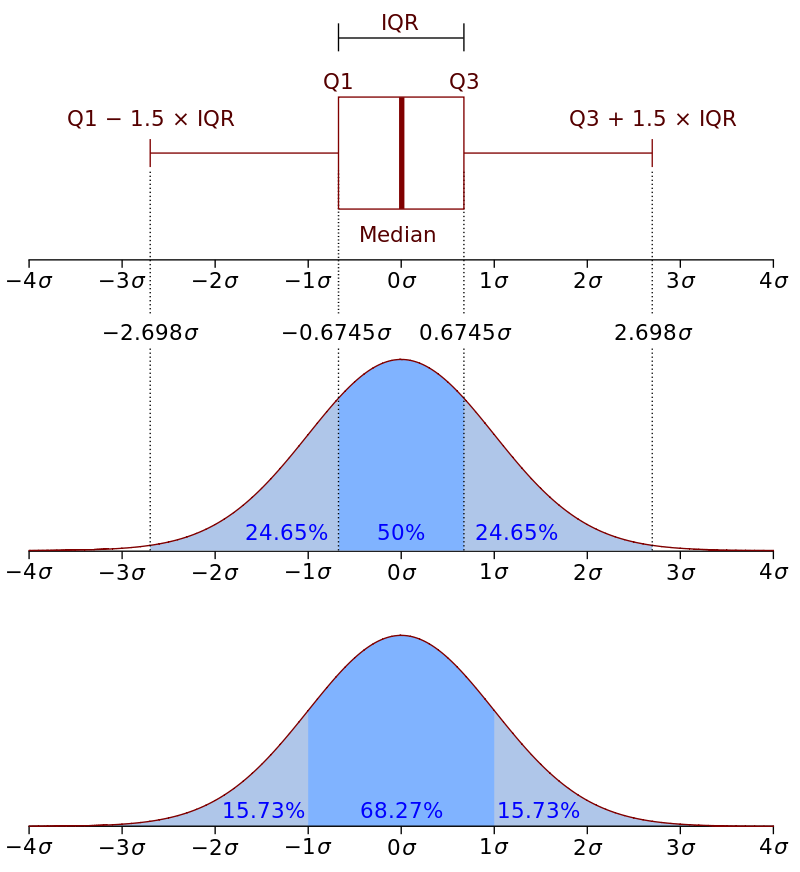
\includegraphics[width=0.7\linewidth]{../Assets/pdfplot}
		\caption{Probability density function of a normal distribution}
		\label{fig:pdfplot}
	\end{figure}
	
\subsubsection{Performance evaluation}
	Estimating the number of mesh nodes and the time steps required to implement DNS and LES shows the complexity of the problem from a computational point of view.
	
	\begin{table}[H]
		\begin{center}
			\begin{tabular}{|c|c|c|c|c|}
				\hline
				Method & Number of nodes & Number of time steps & Year\\
				\hline
				RANS & $10^7$ & $10^3$ & 1985\\
				\hline
				DES & $10^8$ & $10^4$ & 2000\\
				\hline
				LES & $10^{11.5}$ & $10^{6.7}$ & 2045\\
				\hline
				DNS & $10^{16}$ & $10^{7.7}$ & 2080\\
				\hline
			\end{tabular}
		\end{center}
		\caption{Perspective of application of methods}
	\end{table}
	Year means the practical application of the method with the time spent no more than a day.
	To estimate the required computing resources (for example, speed and amount of RAM), we take a computational grid of 100$\times$100$\times$100 nodes ($10^6$ points). At each node, it is necessary to calculate about 10 functions (velocity components, density, pressure, temperature, turbulence characteristics, concentrations of mixture components). The values of unknown functions are found as a result of solving a system of nonlinear equations, which requires from 200 to 1000 arithmetic operations. It is necessary to perform $10^{10}$ floating point operations in one time step. To study the development of the process in time, up to 1000 time steps are required. As a result, performing one calculation requires $10^{13}$ floating point operations. A computer with a performance of 100 MFlops ($10^8$ floating point operations per second) will spend $10^7$ seconds to perform one computational variant. To carry out the calculation in 100 minutes, you will need a computer with a performance of 0.1 TFlops.
	\newpage
	\section{Modeling using ANSYS FLUENT}
	\subsection{Formulation of the problem}
	The initial velocity at the entrance to the channel is $U_0 = 0.29$ m/s.
	At the exit from the channel, the condition of equality to zero of the derivative along the normal to the boundary is set.
	\begin{equation}
		\frac{\partial}{\partial n} = 0
	\end{equation}
	The no-flow and no-slip boundary conditions are set for the wall. This is expressed by the equality to zero of the normal and tangential velocity components.
	\begin{equation}
		v \cdot n = 0 \qquad v \cdot \tau = 0
	\end{equation}
	Here $n$ and $\tau$ are the unit vectors of the normal and tangent to the channel surface. The boundary conditions for the pressure are set by discretizing the equation for the change in momentum in the projection onto the normal to the wall.
	
	The wall restrains the growth of small eddies and changes the mechanism of energy exchange between resolvable and insoluble turbulence scales. In this case, the number of grid nodes required to calculate the flow in the boundary layer increases to a value characteristic of DNS. In order to reduce the consumption of computing resources and take into account the influence of various factors, such as surface roughness, the near-wall function method and various models of the turbulent boundary layer are used\cite{Cabot2000}.
\subsection{Visualization of the task}
	Built-in ANSYS tools were used to build the channel geometry and create a grid model.
\subsubsection{Channel geometry}
	The object of study is a turbulent boundary layer in a channel. The channel is divided into two parts. The first part is a narrowing from 369.5$\times$149.8 mm at the beginning to 124$\times$50 mm. The length of this section is 396 mm. It allows you to significantly increase the flow rate of the liquid. The second part is straight, 1100 mm long.
	\begin{figure}[H]
		\centering
		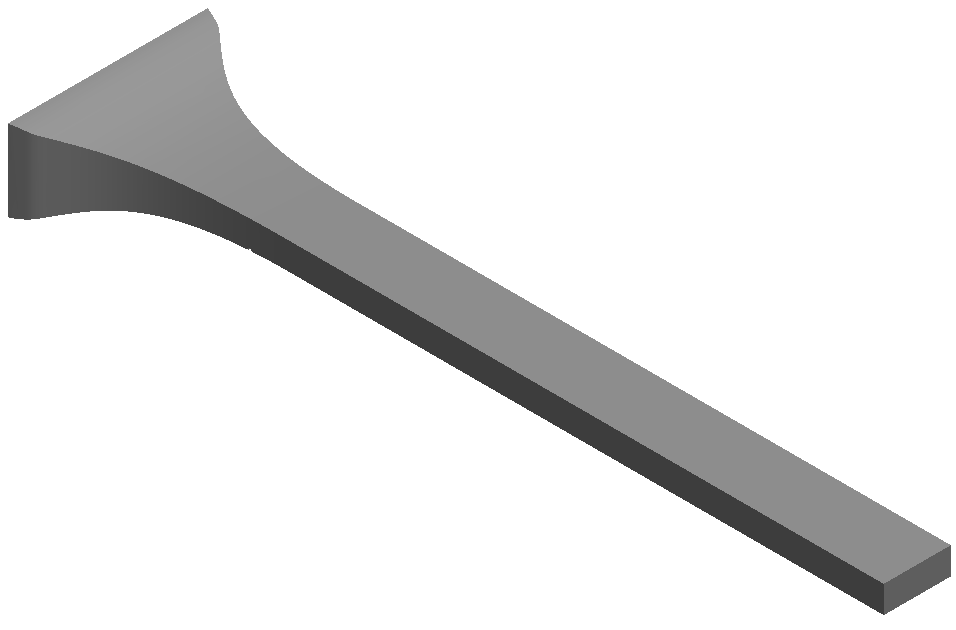
\includegraphics[width=0.7\linewidth]{../Assets/ВидКанала1}
		\caption{\footnotesize{General view of the channel}}
		\label{fig:channelview}
	\end{figure}
	At a distance of 323.9 mm from the entrance to the channel, at the base there is a cutout representing a wire with a radius of 2.1 mm and a height of 1.98 mm. This obstacle creates a turbulent state.
	\begin{figure}[H]
		\centering
		
\includegraphics[width=0.6\linewidth]{../Assets/ВидКанала4}
		\caption{\footnotesize{Type of obstacle in the channel}}
		\label{fig:vortexgeneratorview}
	\end{figure}
\subsubsection{Building a grid model}
	There are several methods for modeling mesh models in Ansys that can be used depending on the type and size of the model.
	
	The first is the spatial partitioning method, which is often used to model rigid bodies. This method consists of breaking an object into smaller elements called leaf elements. Each finite element is then approximated with simpler shapes such as triangles or rectangles to create a mesh.
	
	The second is a node-based mesh generation method. In this method, the model is represented as a set of nodes connected by lines or surfaces. The mesh is then built based on this structure.
	
	The third is the multiple division method. This method is often used to model spatial objects such as aircraft or cars. It consists in breaking the object into smaller blocks and then dividing each block into even smaller blocks. Each block is then approximated with simpler shapes to create a mesh.
	\begin{figure}[H]
		\centering
		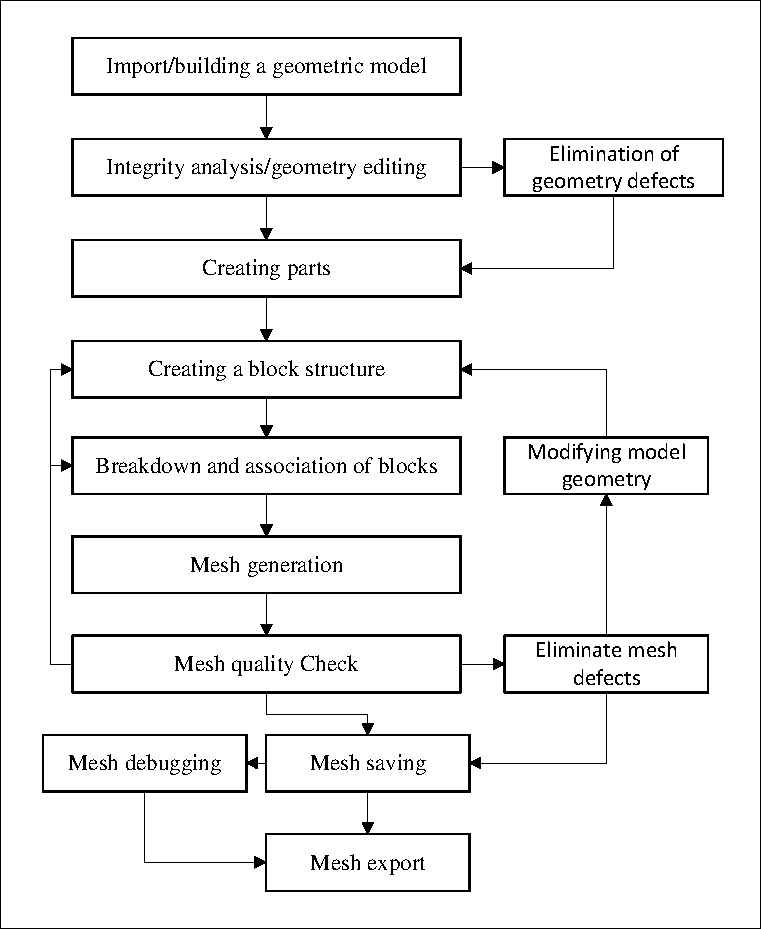
\includegraphics[width=0.7\linewidth]{../Assets/СхемаСозданияСеткиEN}
		\caption{\footnotesize{The scheme of work on the grid model}}
		\label{fig:meshScheme}
	\end{figure}
	The figure \ref{fig:meshScheme} shows a schematic plan for generating a mesh. This method is the most optimal for building a sufficiently high-quality grid model. Dividing the geometry into parts allows you to speed up the construction by parallel distribution of calculations (one core is allocated for each part). In addition, disabling the multithreading mode (one physical core is divided into two virtual ones) for the processor increases performance, since all the power of the core is used, and not half of it.
	
	As a result of work on the grid model, we managed to achieve the optimal result for calculations. The channel model was divided into 4 blocks. The first block is the entrance to the canal, the second is the section with an obstacle, the third is to the end of the narrowing, the fourth is the straight section of the canal. Mesh statistics: 51397337 nodes and 12665608 elements. The resulting model has a compaction towards the bottom of the channel, since the boundary layer is of particular importance for the study in this work.
	\begin{figure}[H]
		\centering
		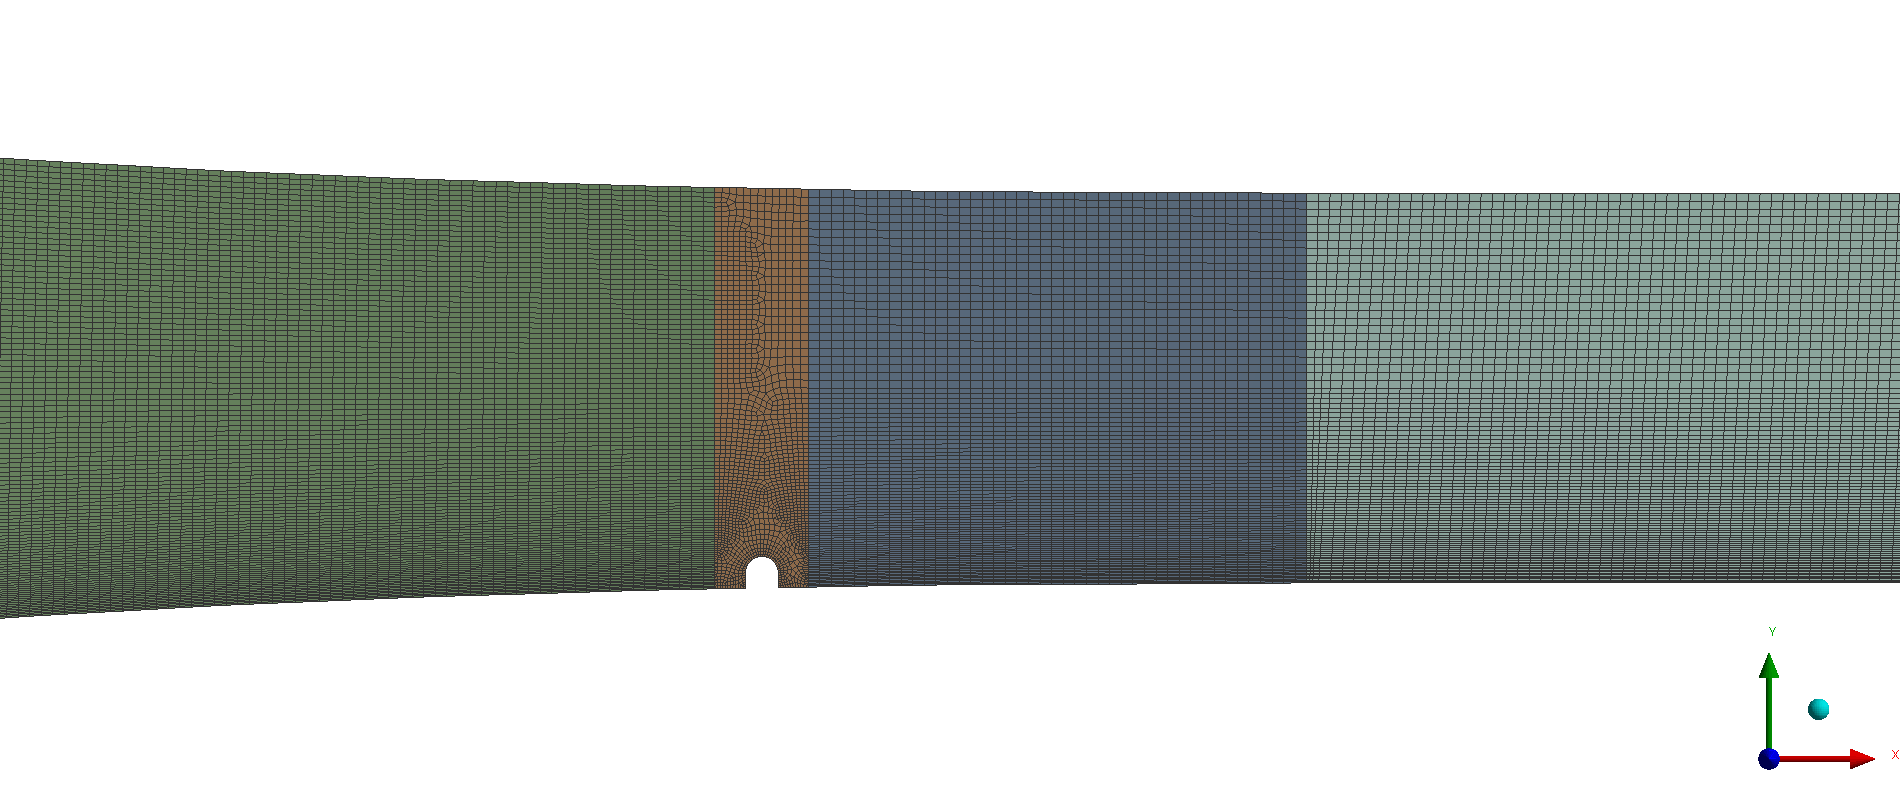
\includegraphics[width=1\linewidth]{../Assets/Mesh1}
		\caption{\footnotesize{Mesh}}
		\label{fig:mesh1}
	\end{figure}
	
\subsection{Calculation in ANSYS Fluent}
	Ansys Fluent is a general-purpose computational fluid dynamics (CFD) software used to model fluid flow, heat and mass transfer, chemical reactions, and more. Fluent offers a modern, user-friendly interface that streamlines the CFD process from pre- to post-processing within a single window workflow. Fluent is known for its advanced physics modeling capabilities, which include turbulence modeling, single and multiphase flows, combustion, battery modeling, fluid-structure interaction, and much more. Also known for its efficient HPC scaling, large models can easily be solved in Fluent on multiple processors on either CPU or GPU. Multiple solver options are available, including pressure-based and density-based CPU solvers to cover low-speed to hypersonic flows and a pressure-based native GPU solver.
	
	Water was used as a liquid with the following characteristics: $\rho = 998.2$ $kg/m^3$ and $\nu = 0.001003$ $kg/m\cdot s$. For the subgrid model of the LES method, the WALE model was used with the coefficient $C_w = 0.325$. The main advantages of this model:
	\begin{itemize}
		\item the spatial operator contains both local deformations and rotational velocities. Thus, all turbulence structures related to the dissipation of kinetic energy are calculated by this model;
		\item the turbulent viscosity tends naturally to zero near the wall, so that neither a constant (dynamic) adjustment nor a damping function is required to calculate wall-bounded flows;
		\item the model gives zero turbulent viscosity in pure shear. Thus, it can reproduce the process of transition from laminar to turbulent flow due to the growth of linear unstable regimes.
	\end{itemize}
	In addition, the WALE model is invariant to any translation or rotation of coordinates, and only local information is required (no check-filter operation and no knowledge of nearest points in the grid), so it is well suited for LES in complex geometries\cite{Nicoud1999}.
	
	Parameters related to the calculation of equations:
	\begin{table}[H]
		\begin{center}
			\begin{tabular}{|c|c|}
				\hline
				Parameters & Method\\
				\hline
				Scheme & SIMPLEC \\
				\hline
				Gradient & Least squares cell based\\
				\hline
				Pressure & Second order\\
				\hline
				Momentum & Bounded central differencing\\
				\hline
				Time & Bounded second order implicit\\
				\hline
			\end{tabular}
		\end{center}
		\caption{\footnotesize{Solver options}}
	\end{table}
	With the settings and parameters described above, the calculation was launched in ANSYS FLUENT. The time step size is $\Delta t = 0.001 s$, their number is $s_t = 10000$. $s_i = 50$ iterations were calculated for each step. This is 10s real time.
	\newpage
	\section{Analysis of data}
	\subsection{Data processing}
	As a result of the calculations, which took about a month, $.dat$ files were obtained. Each of these data arrays corresponds to a certain time step. For post processing and plotting based on them, the built-in ANSYS CFD-Post tool was used. To analyze the effect of vortex generators on local friction and transfer, different sections were used in different parts of the channel. Some of them are shown on the figure \ref{fig:planesforanalysis}. 
	\begin{figure}[H]
		\centering
		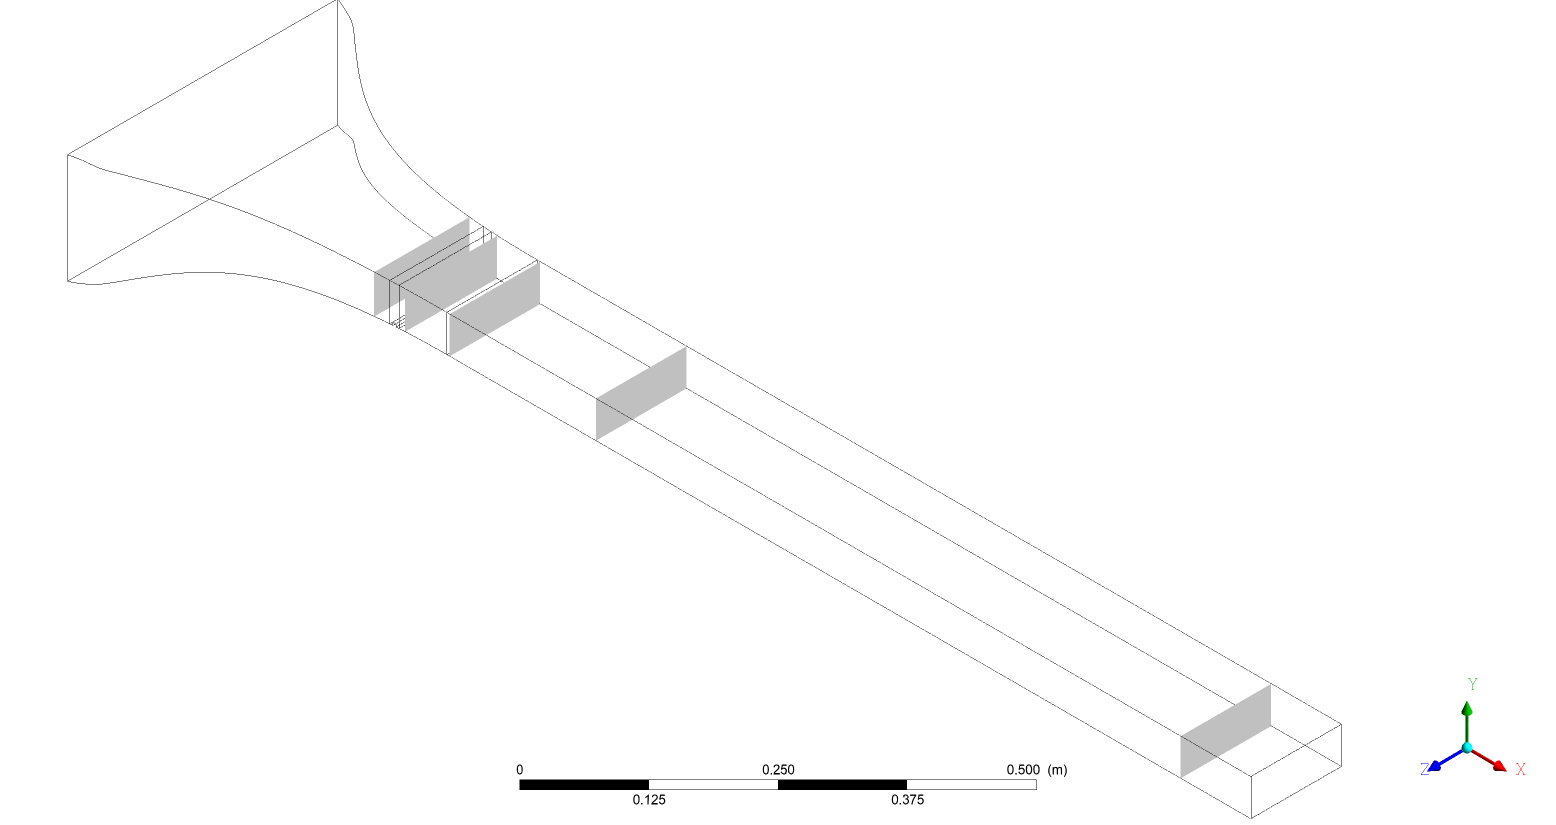
\includegraphics[width=0.9\linewidth]{../Assets/1}
		\caption{Sections for analysis}
		\label{fig:planesforanalysis}
	\end{figure}
	
	The origin of the coordinate axes of the model is located in the center of the channel entrance. Sections were considered at different heights along and at different distances from the entrance to the channel. The table below shows a list of sections, their location and description. Images in applications have names based on the table.
	\begin{table}[H]
		\begin{center}
			\begin{tabular}{|c|c|c|c|}
				\hline
				Label & Plane & Position & Description\\
				\hline
				PlaneXY & XY & Z = 0 & along the whole channel\\
				\hline
				PlaneYZ300 & YZ & X = 300 & in front of the barrier\\
				\hline
				PlaneYZ340 & YZ & X = 340 & after the barrier\\
				\hline
				PlaneYZ400 & YZ & X = 400 & begin of the straight section\\
				\hline
				PlaneYZ600 & YZ & X = 600 & further down the channel\\
				\hline
				PlaneYZ1400 & YZ & X = 1400 & at the exit of the channel\\
				\hline
				PlaneXZ0 & XZ & Y = 0 & above the boundary layer\\
				\hline
				PlaneXZ20M & XZ & Y = -20 & above the barrier\\
				\hline
				PlaneXZ23М & XZ & Y = -23 & at the barrier level\\
				\hline
			\end{tabular}
		\end{center}
		\label{tbl:sections}
		\caption{List of sections}
	\end{table}
	
	After the completion of the calculations, a graph was automatically generated, thanks to which it is possible to evaluate the accuracy of the results obtained on this grid model. It reached a value of $10^{-3}$.
	\begin{figure}[H]
		\centering
		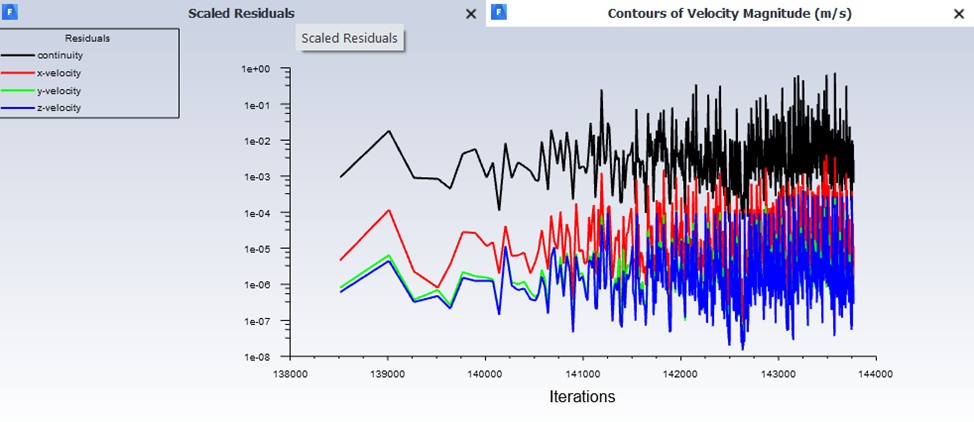
\includegraphics[width=1\linewidth]{../Assets/scaledResiduals}
		\caption{Scaled residuals}
		\label{fig:scaledresiduals}
	\end{figure}
\subsection{Influence on local friction and transport}
	Further, for the convenience of describing the results and their evaluation, several points are presented on various parameters.
\subsubsection{Velocity}
	Let's start with velocity. According to the obtained sections, the contours of average velocity were constructed for various time intervals.
	\begin{figure}[H]
		\centering
		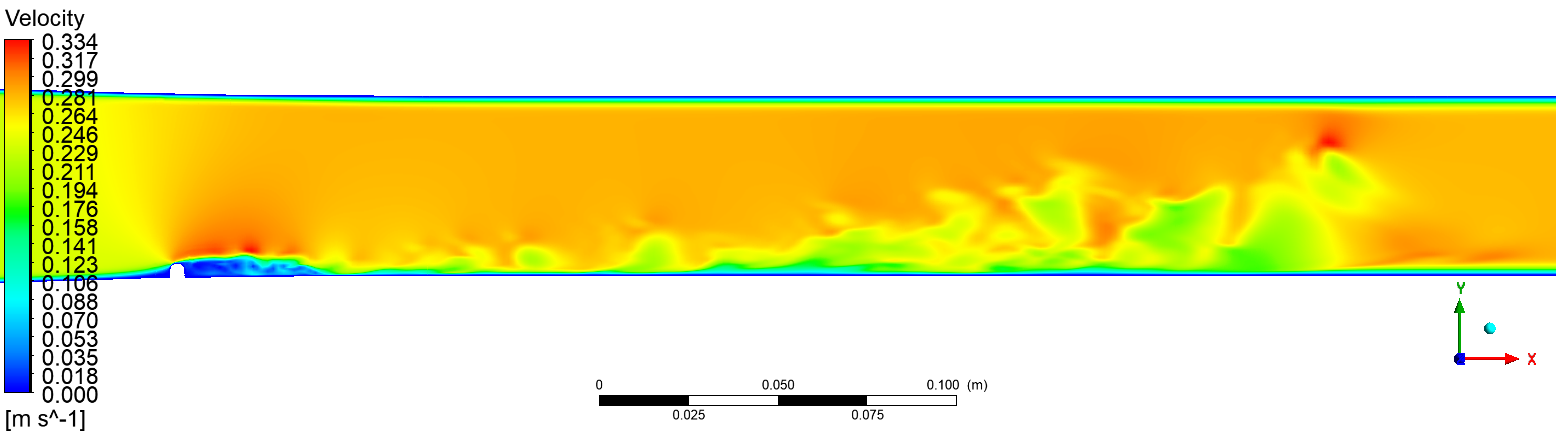
\includegraphics[width=1\linewidth]{../Assets/T16_Velocity_ContourXY}
		\caption{Velocity in longitudinal section XY, t = 1.6 c}
		\label{fig:t16velocitycontourxy}
	\end{figure}
	As can be seen from the figure along the channel, the velocity immediately behind the obstacle and at its level approached zero. And over the wire has increased significantly. Due to such abrupt changes in speed, vortex structures are formed, the speed of which is clearly visible in these images.
	
	\begin{figure}[H]
		\begin{subfigure}{.5\textwidth}
			\centering
			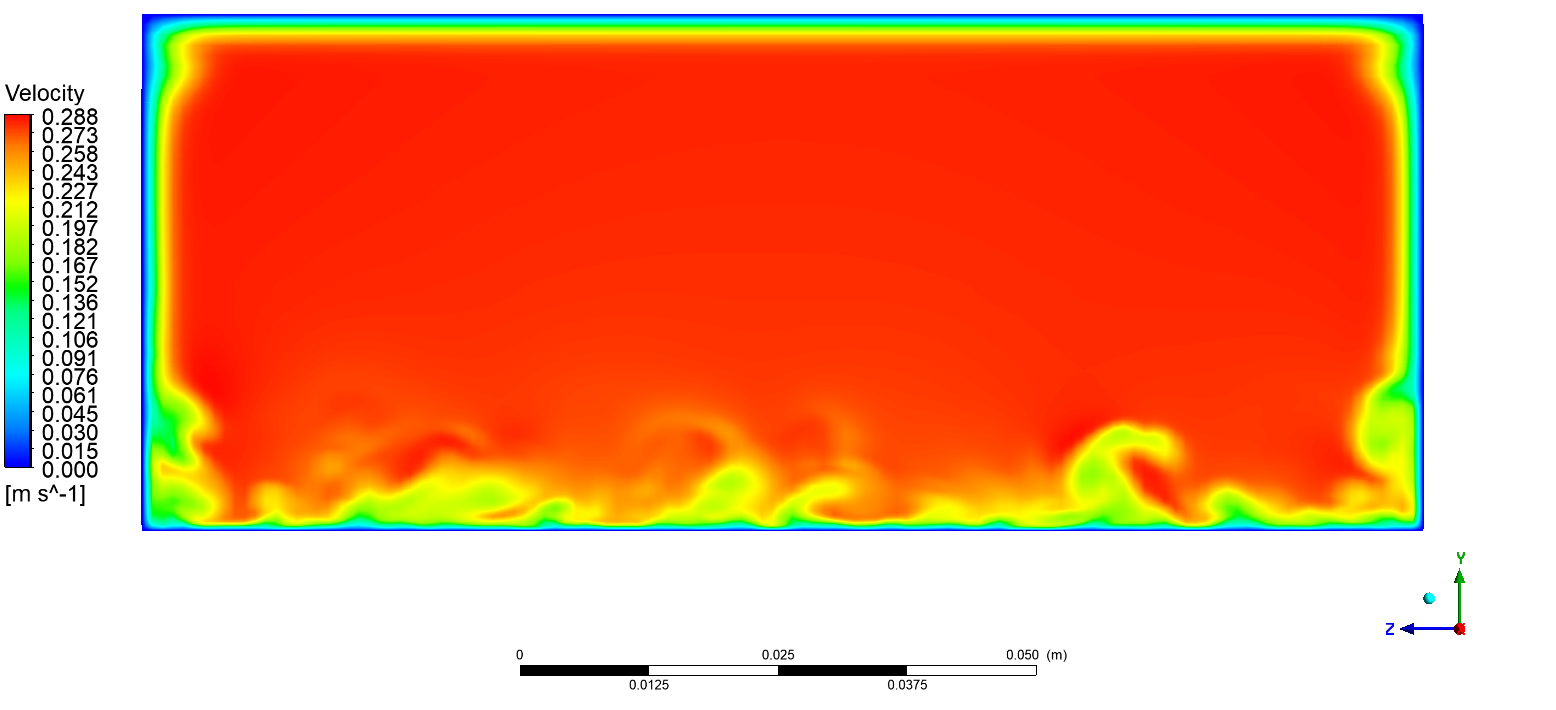
\includegraphics[width=1.1\linewidth]{../Assets/T16_Velocity_ContourYZ400}
			\caption{PlaneYZ400}
			\label{fig:T16VelocityContourYZ340}
		\end{subfigure}%
		\begin{subfigure}{.5\textwidth}
			\centering
			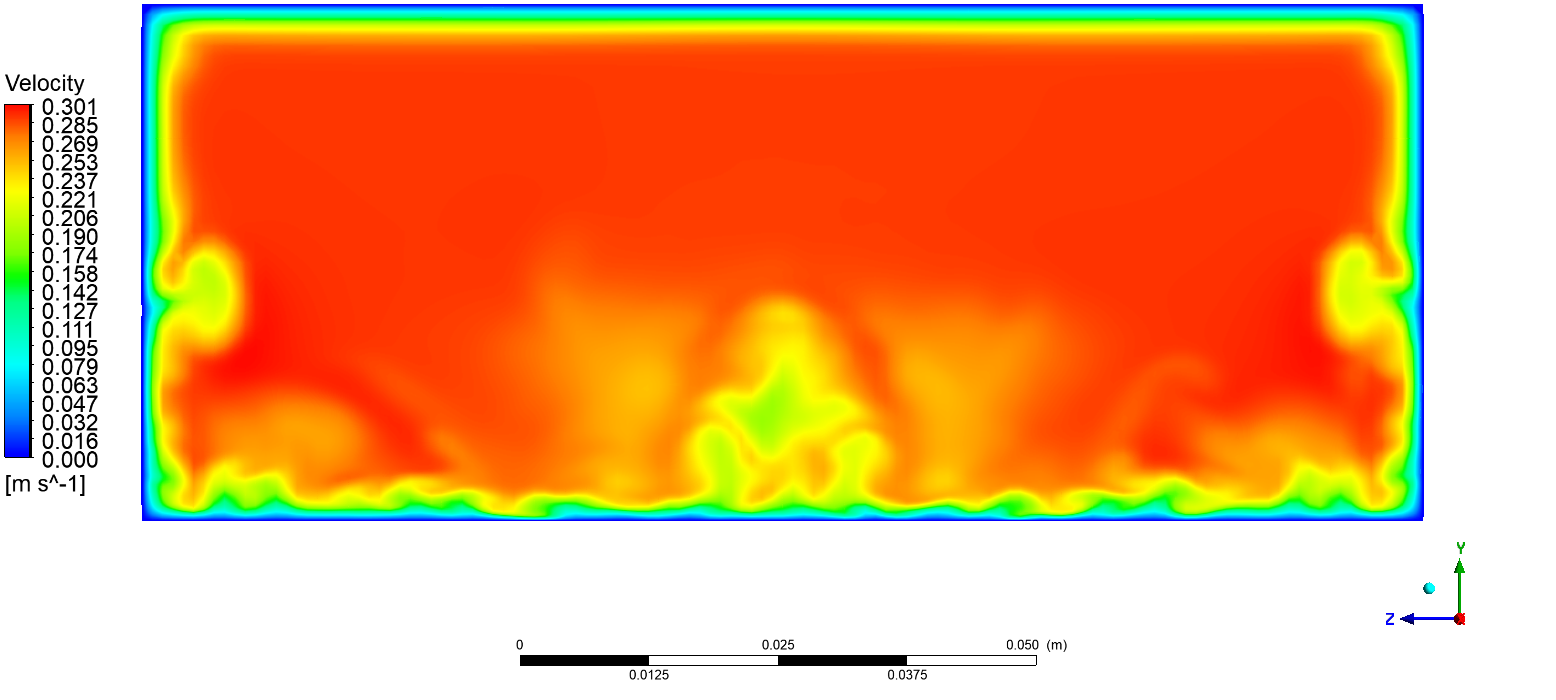
\includegraphics[width=1.1\linewidth]{../Assets/T16_Velocity_ContourYZ600}
			\caption{PlaneYZ600}
			\label{fig:T16VelocityContourYZ400}
		\end{subfigure}
		\caption{Velocity in cross sections at t = 1.6 с}
		\label{fig:T16VelocityContourYZ}
	\end{figure}
	These vortex formations can also be seen in figure \ref{fig:T16VelocityContourYZ}. 
	
	\begin{figure}[H]
		\centering
		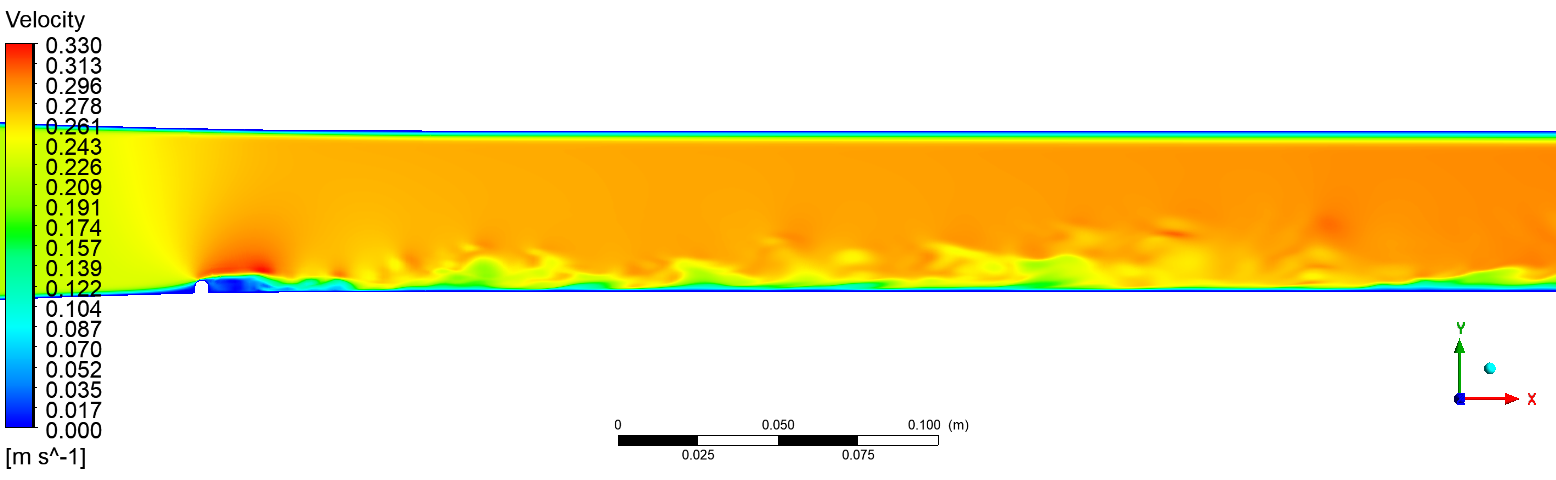
\includegraphics[width=1\linewidth]{../Assets/T96_Velocity_ContourXY}
		\caption{Longitudinal velocity in XY, t = 9.6 с}
		\label{fig:t96velocitycontourxy}
	\end{figure}
	By the time t = 9.6 s, the vortex structure of the channel became less visible and large eddies were transformed into small ones.
	Let us consider more detail velocity in cross sections at time t = 9.6 s.
	\begin{figure}[H]
		\begin{subfigure}{.5\textwidth}
			\centering
			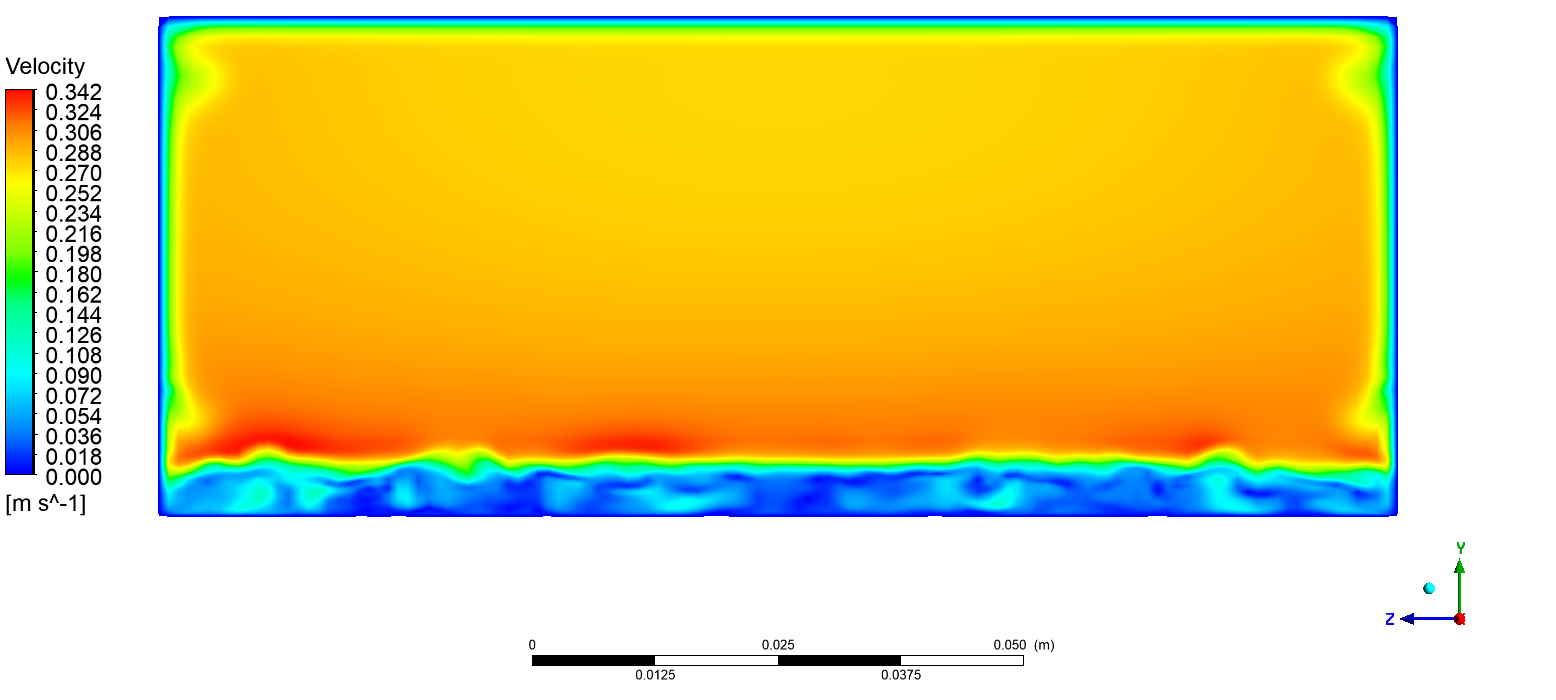
\includegraphics[width=1.1\linewidth]{../Assets/T96_Velocity_ContourYZ340}
			\caption{PlaneYZ340}
			\label{fig:T96VelocityContourYZ340}
		\end{subfigure}%
		\begin{subfigure}{.5\textwidth}
			\centering
			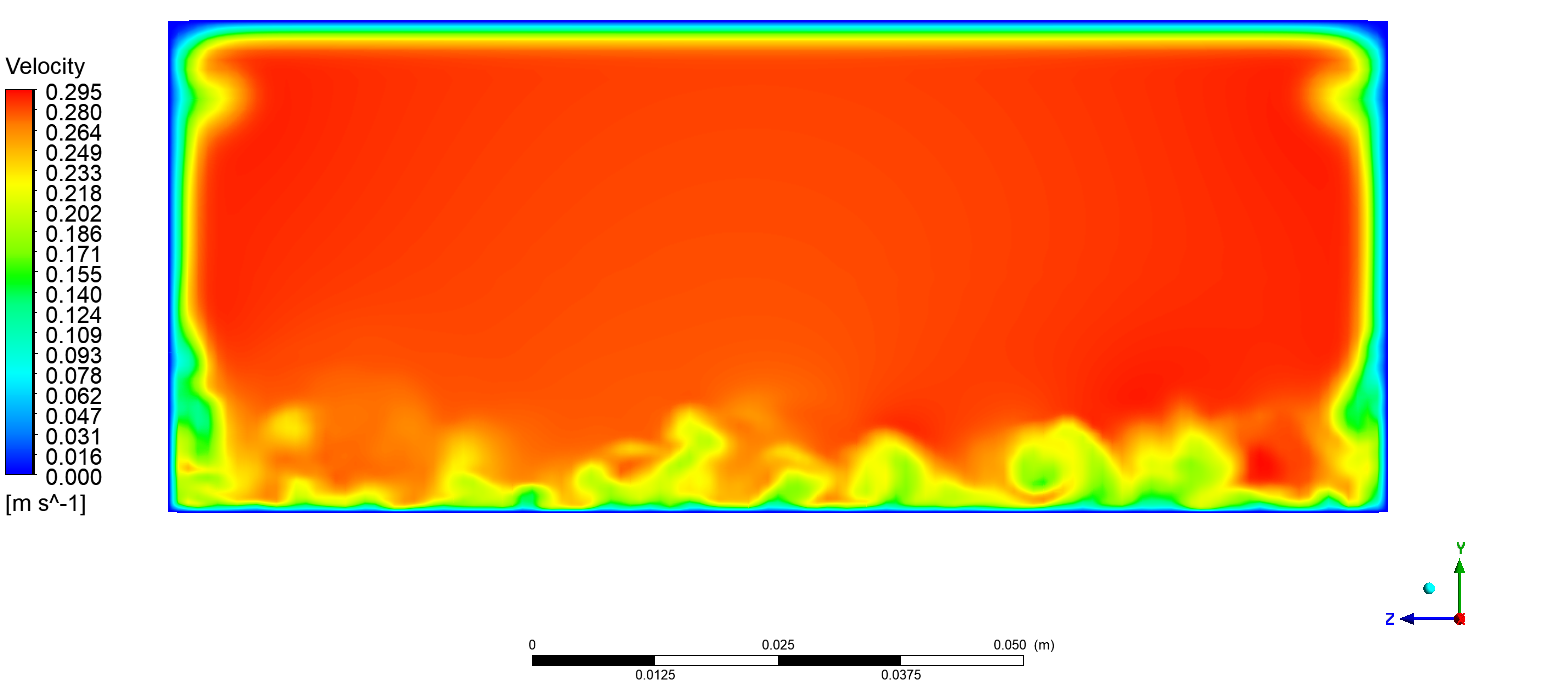
\includegraphics[width=1.1\linewidth]{../Assets/T96_Velocity_ContourYZ400}
			\caption{PlaneYZ400}
			\label{fig:T96VelocityContourYZ400}
		\end{subfigure}
		\\
		\begin{subfigure}{.5\textwidth}
			\centering
			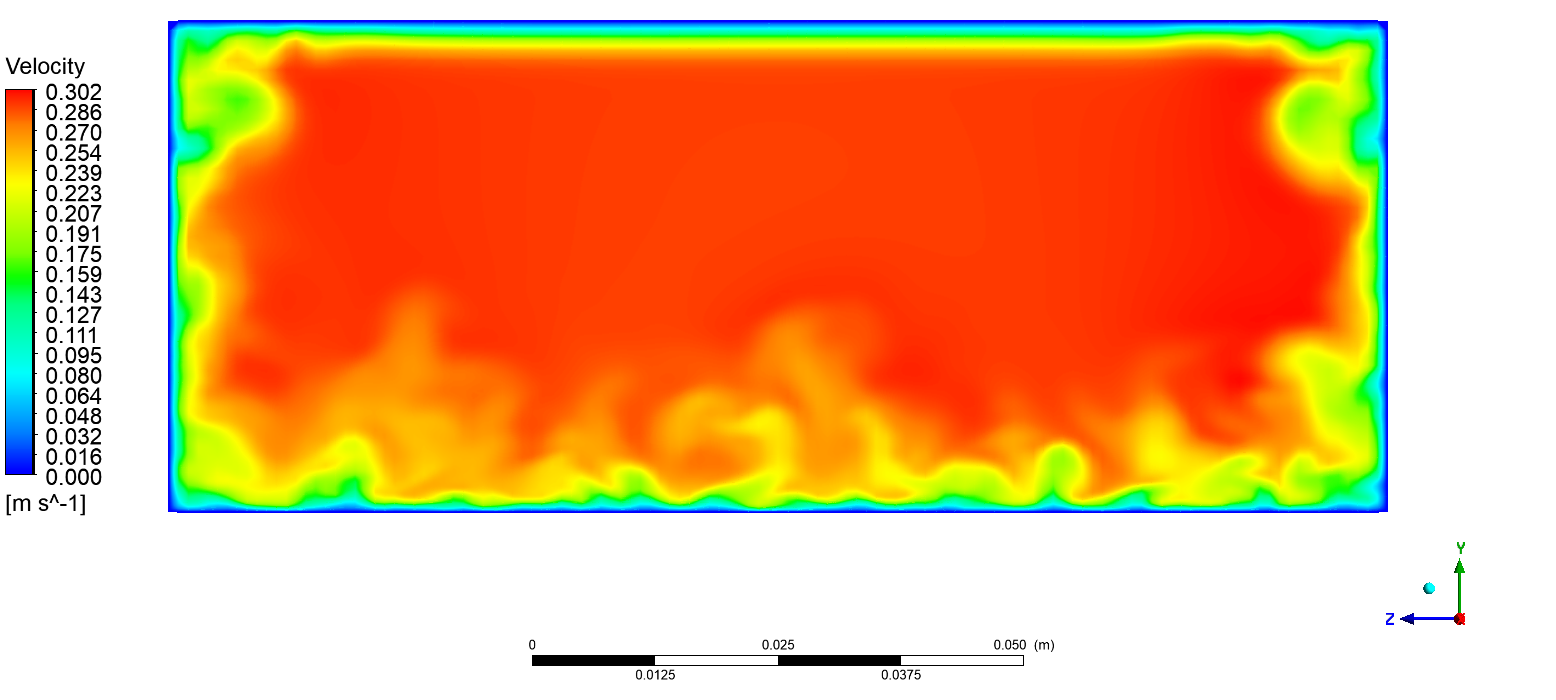
\includegraphics[width=1.1\linewidth]{../Assets/T96_Velocity_ContourYZ600}
			\caption{PlaneYZ600}
			\label{fig:T96VelocityContourYZ600}
		\end{subfigure}%
		\begin{subfigure}{.5\textwidth}
			\centering
			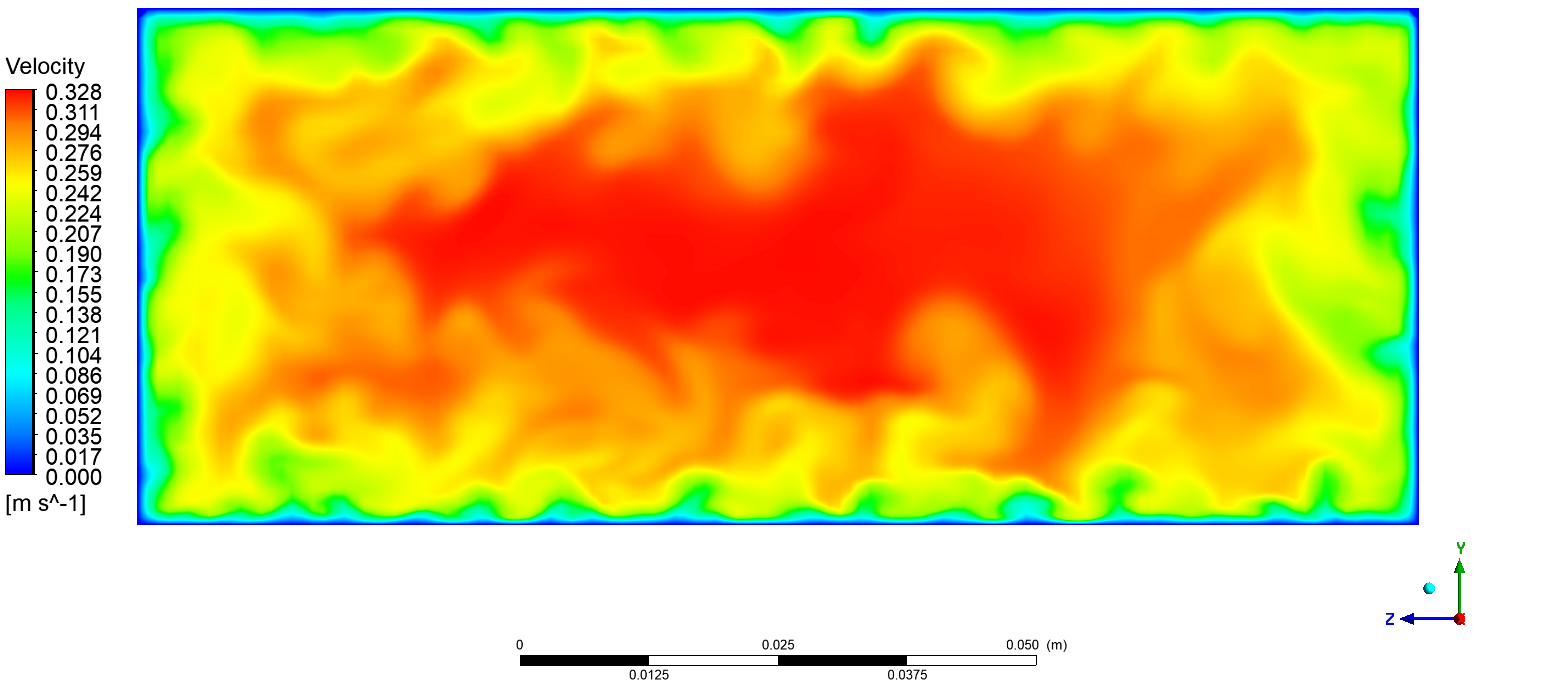
\includegraphics[width=1.1\linewidth]{../Assets/T96_Velocity_ContourYZ1400}
			\caption{PlaneYZ1400}
			\label{fig:T96VelocityContourYZ1400}
		\end{subfigure}
		\caption{Velocity in cross sections at t = 9.6 с}
		\label{fig:T96VelocityContourYZ}
	\end{figure}
	As seen in the picture \ref{fig:T96VelocityContourYZ} the formed vortices gradually decay to Kolmagorov scale vortices and dissipate into energy.
	
	\begin{figure}[H]
		\begin{subfigure}{1\textwidth}
			\centering
			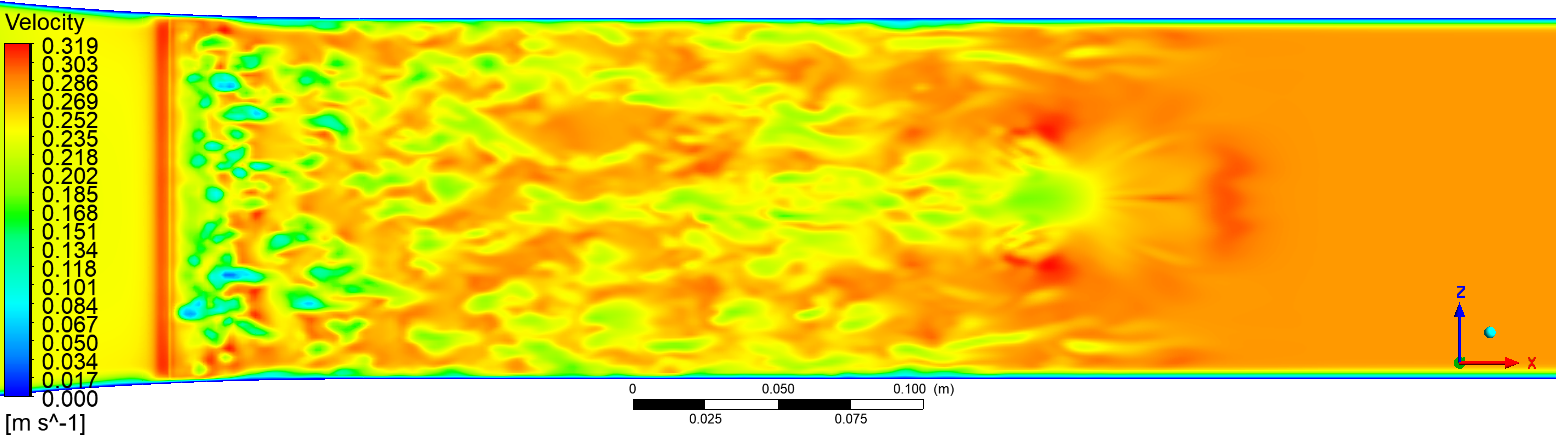
\includegraphics[width=1\linewidth]{../Assets/T16_Velocity_ContourXZ20M}
			\caption{PlaneXZ20M}
			\label{fig:T16VelocityContourXZ20M}
		\end{subfigure}%
		\\
		\begin{subfigure}{1\textwidth}
			\centering
			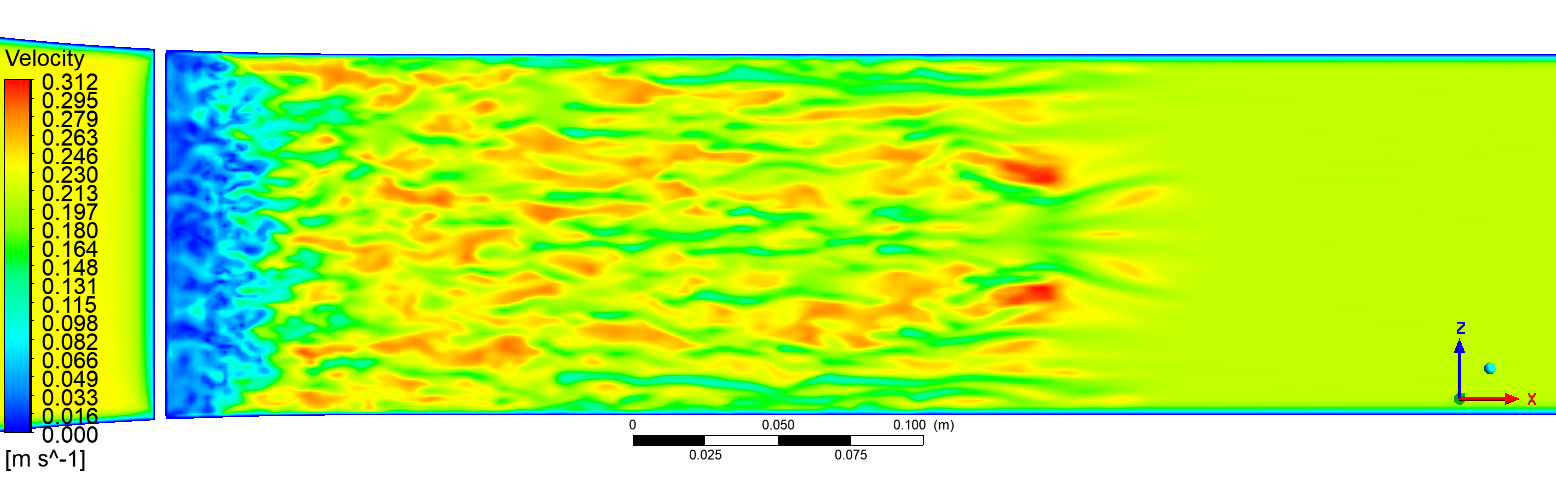
\includegraphics[width=1\linewidth]{../Assets/T16_Velocity_ContourXZ23M}
			\caption{PlaneXZ23M}
			\label{fig:T16VelocityContourXZ23M}
		\end{subfigure}
		\caption{Speed in longitudinal sections XZ at t = 1.6 с}
		\label{fig:T16VelocityContourXZ}
	\end{figure}
\subsubsection{Friction coefficient}
	In order to obtain friction coefficient data for plotting, the necessary sections were built in Ansys Fluent. They divide the channel lengthwise into 3 parts ($z_1 = -31, z_2 = 0, z_3 = 31$). After that, the built-in tools exported the data to $.csv$ files. Further, with the help of MS Excel, the data concerning the boundary layer were selected. And finally, plots are generated in gnuplot. 
	Four time periods were evaluated. The plots show the dependence of $C_f$ on the coordinate $x$. When the fluid flow reaches an obstacle, $C_f$ changes abruptly. The coefficient increased by 2.6 times. As we moved along the length of the channel, the coefficient decreased and stabilized. This is due to a decrease in the influence of vortex structures on the boundary layer.
	\begin{figure}[H]
		\begin{subfigure}{.5\textwidth}
			\centering
			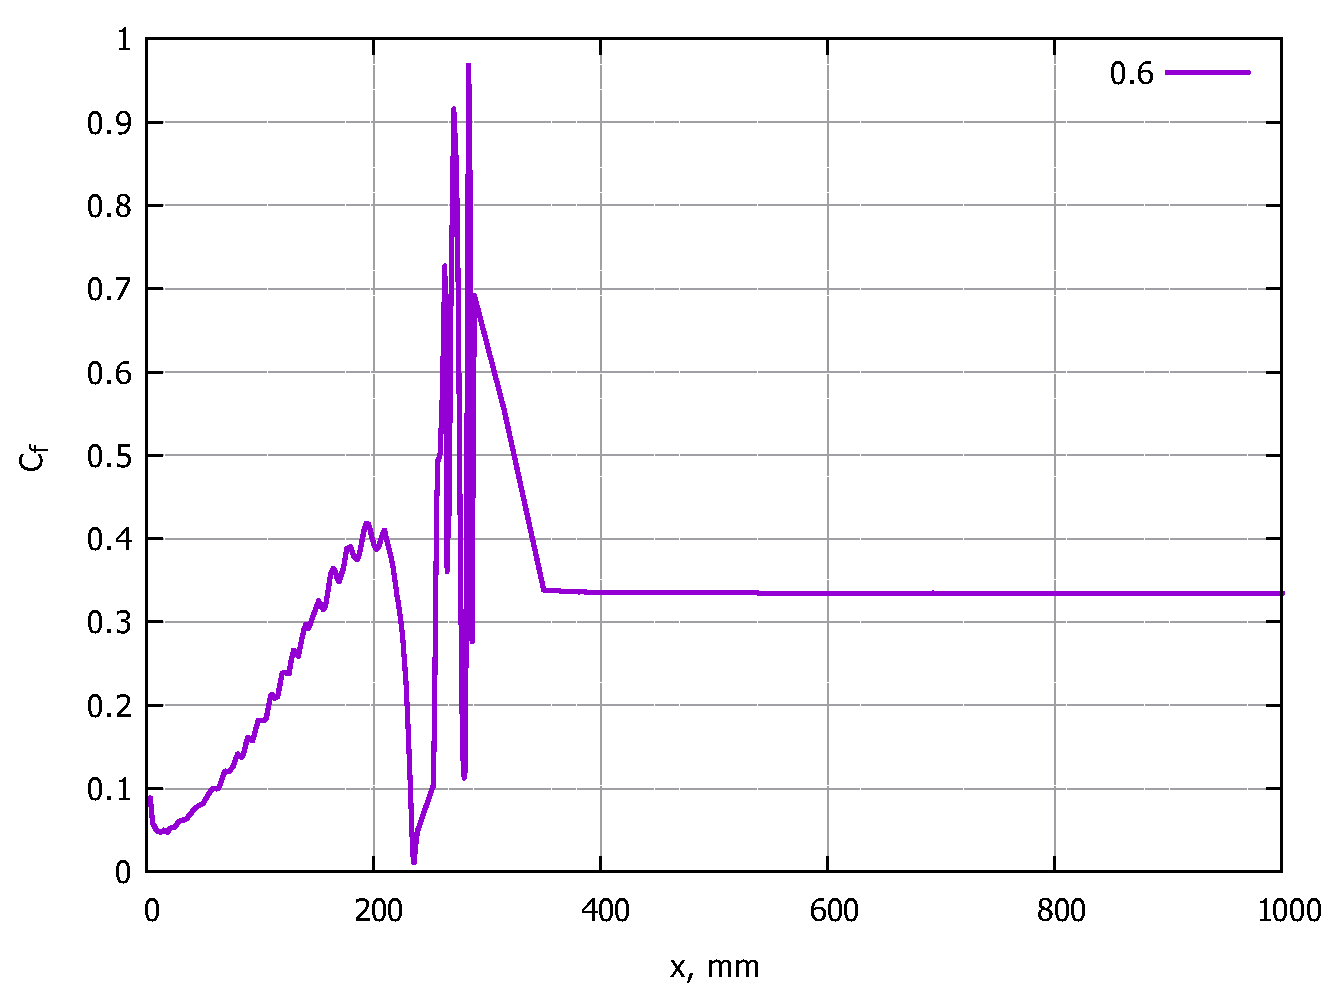
\includegraphics[width=1\linewidth]{../Assets/Cf-T06}
			\caption{t = 0.6 с}
			\label{fig:Cf-T06}
		\end{subfigure}%
		\begin{subfigure}{.5\textwidth}
			\centering
			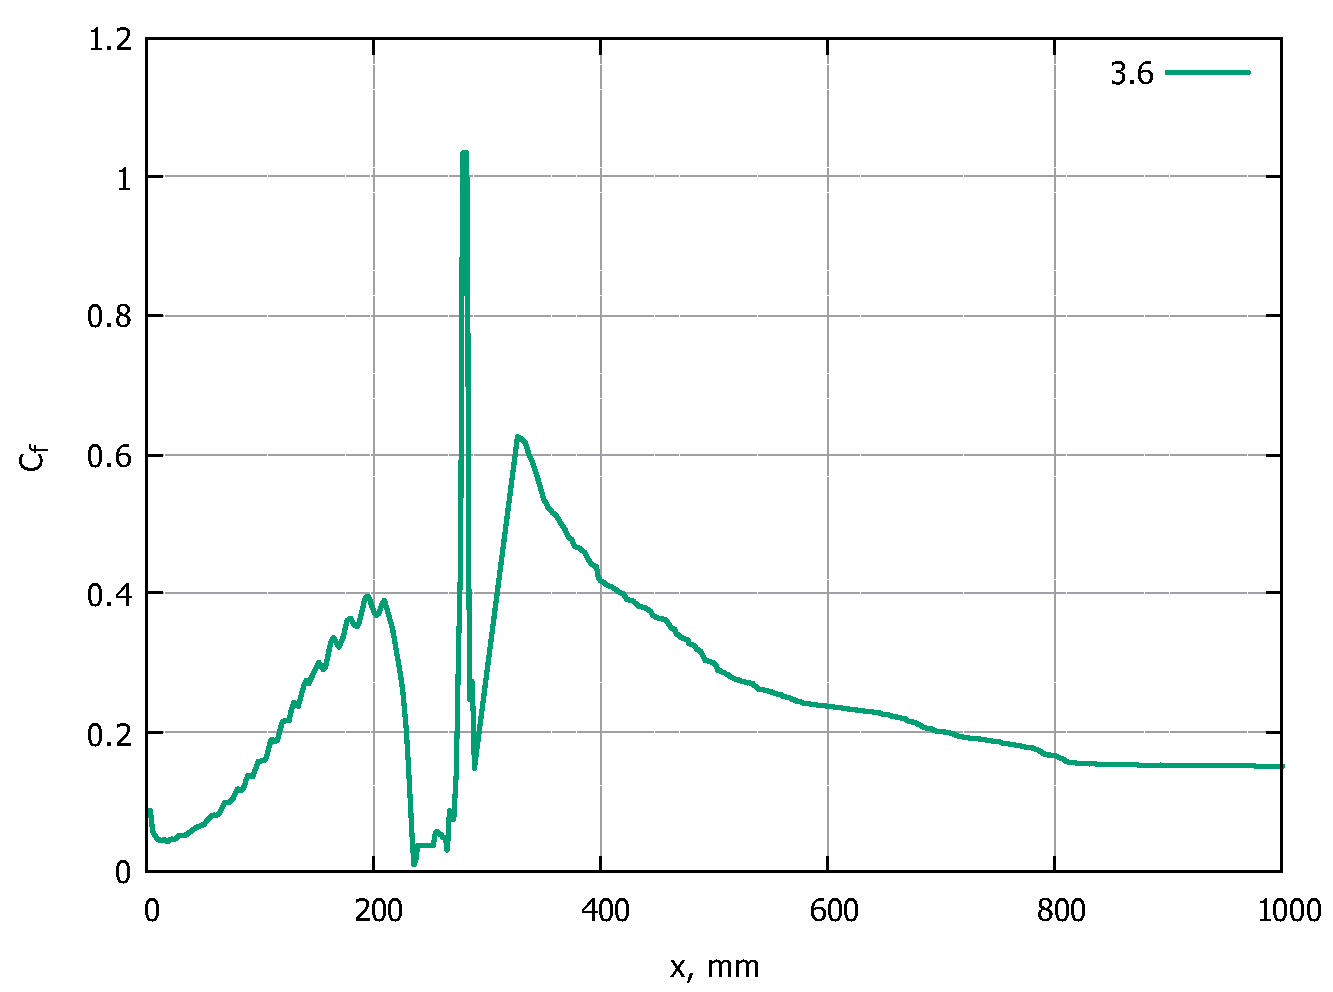
\includegraphics[width=1\linewidth]{../Assets/Cf-T360}
			\caption{t = 3.6 с}
			\label{fig:Cf-T360}
		\end{subfigure}
		\\
		\begin{subfigure}{.5\textwidth}
			\centering
			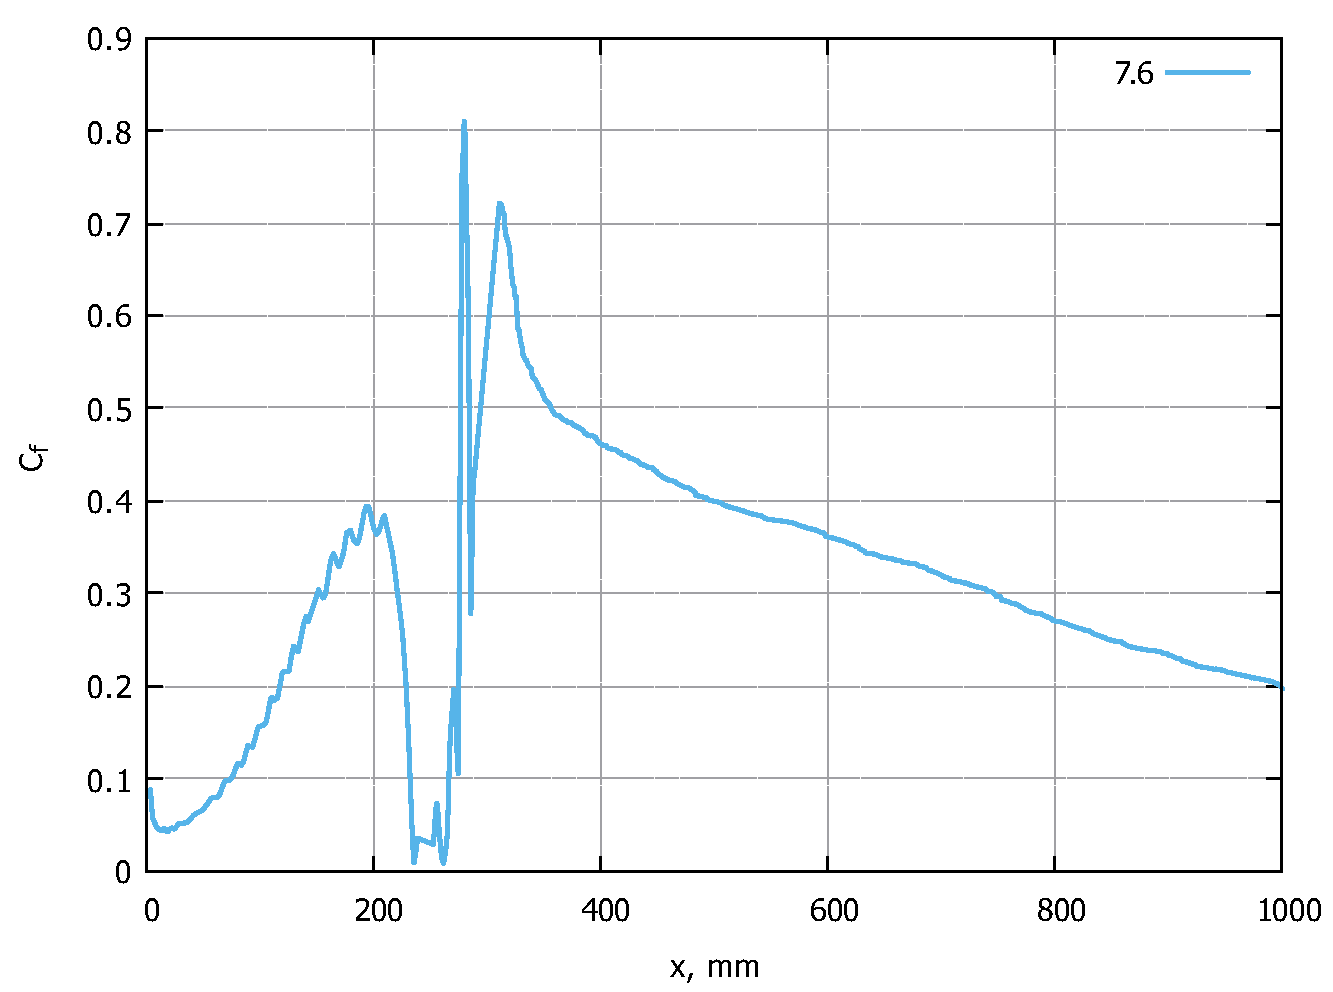
\includegraphics[width=1\linewidth]{../Assets/Cf-T760}
			\caption{t = 7.6 с}
			\label{fig:Cf-T760}
		\end{subfigure}%
		\begin{subfigure}{.5\textwidth}
			\centering
			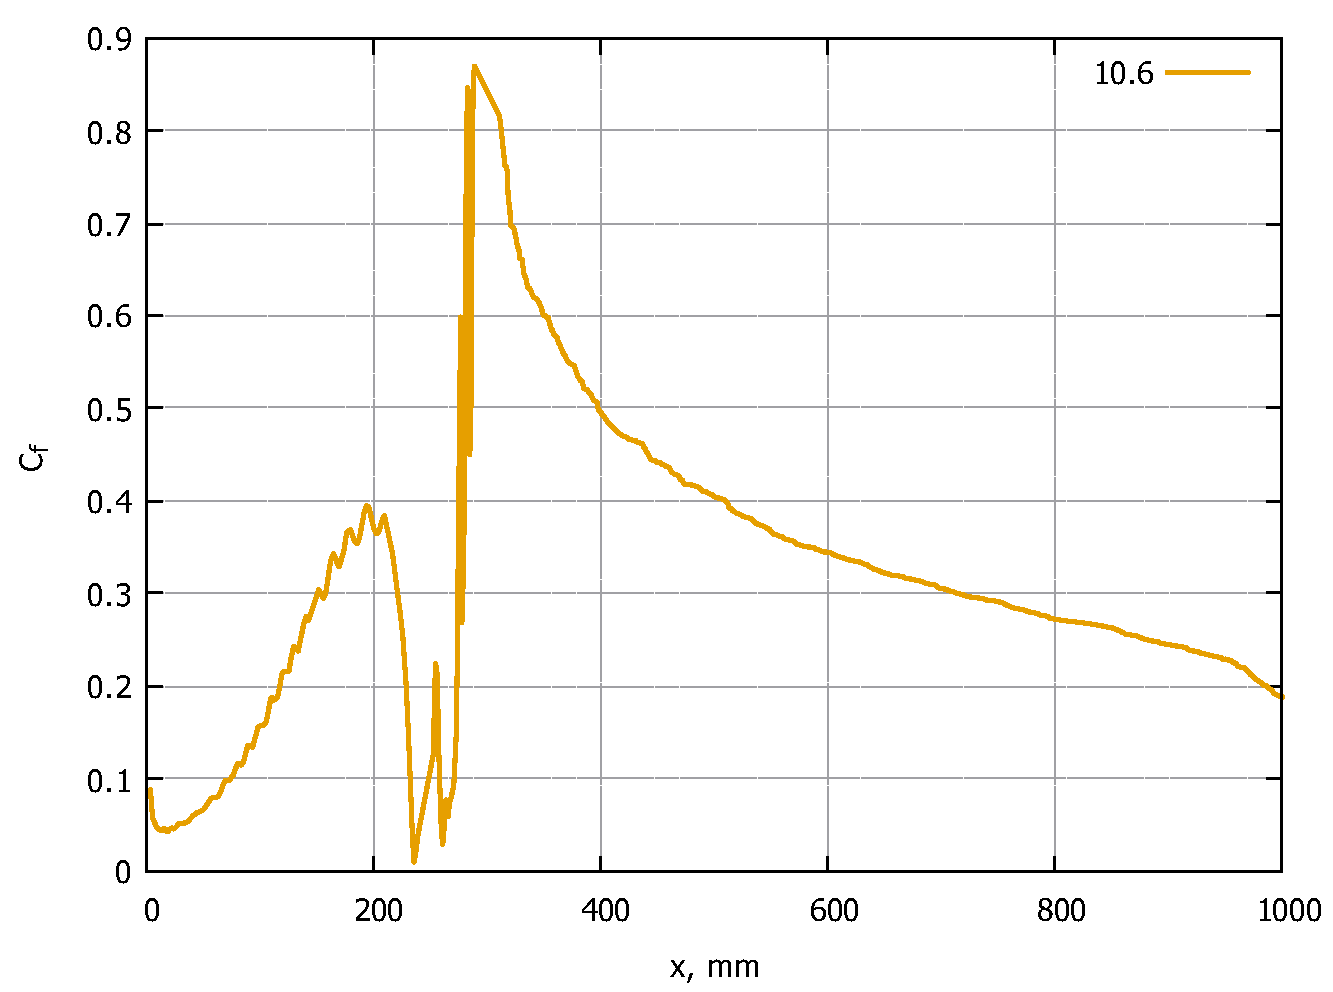
\includegraphics[width=1\linewidth]{../Assets/Cf-T1060}
			\caption{t = 10.6 с}
			\label{fig:Cf-T1060}
		\end{subfigure}
		\caption{Change in the friction coefficient along the length of the channel, z = 0}
		\label{fig:cf}
	\end{figure}
\subsubsection{Q-criterion}
	There are various approaches to the visualization of vortex flows that use one or another definition of a vortex and criteria for its identification. The classification of visualization methods for vortex flows is carried out depending on how the vortex is defined (in the area or on the line), whether the method is invariant with respect to the transformation of the coordinate system, whether the approach is local or global\cite{Hunt1988}. One of these is the $Q$-criterion. It is determined by two components: the strain rate tensor $S$ and the rotation tensor $\Omega$.
	\begin{equation}
		S = \frac{1}{2}(\frac{\partial u_i}{\partial x_j} + \frac{\partial u_j}{\partial x_i}) \qquad \Omega = \frac{1}{2}(\frac{\partial u_i}{\partial x_j} - \frac{\partial u_j}{\partial x_i})
	\end{equation}
	The $Q$-criterion is defined as the second invariant of the velocity gradient tensor\cite{Wiebel2007}.
	\begin{equation}
		Q = \frac{1}{2}(||\Omega||^2 - ||S||^2)
	\end{equation}
	From this we can see that positive values of $Q$ indicate regions in the flow field where vorticity dominates, and negative values of $Q$ indicate regions where strain rate or viscous stress dominates. In addition, there are various versions of the $Q$ criterion in modified expressions that are used to describe different flow regions\cite{Berdahl1993,Chong1990}.
	
	Various areas of eddy formations are presented below. In the figure \ref{fig:q860-t16}, one can notice a clearly expressed structure of the formed vortex.
	\begin{figure}[H]
		\centering
		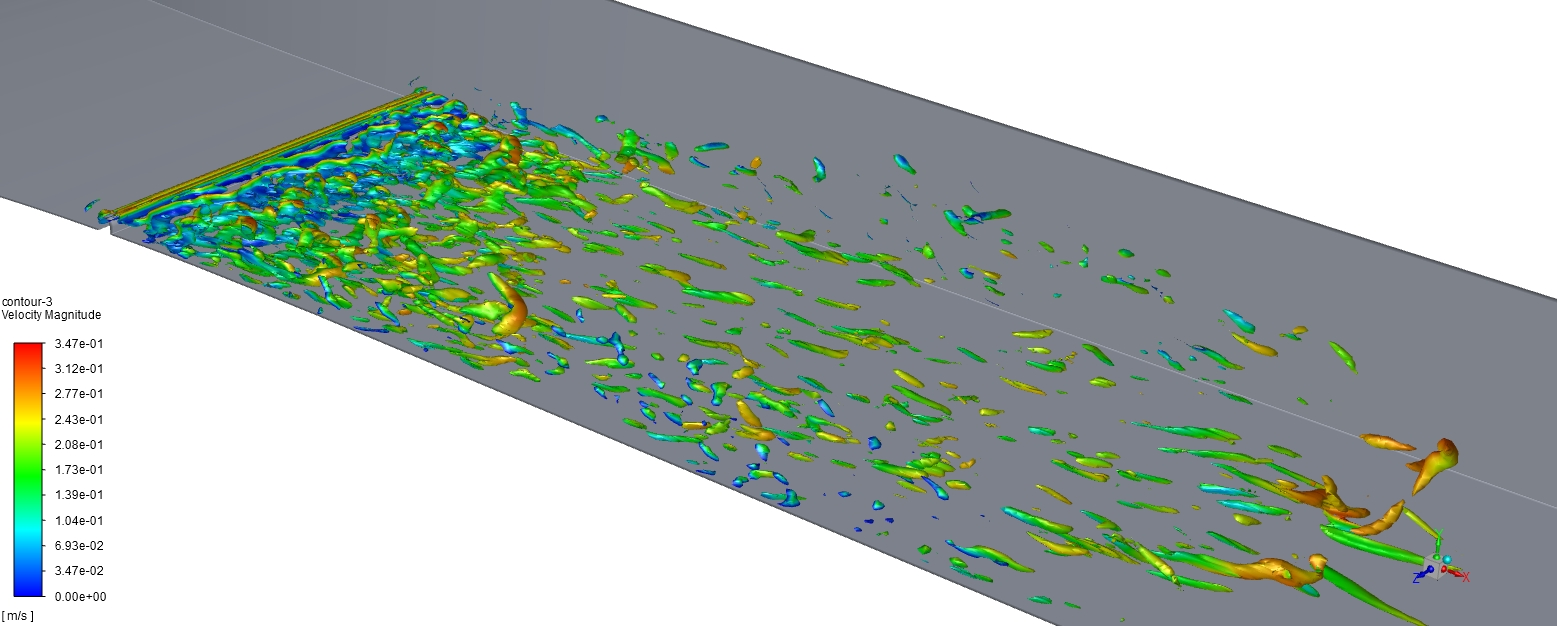
\includegraphics[width=1\linewidth]{../Assets/Q860-t16}
		\caption{Vortex structure at Q = 860 и t = 1.6 c}
		\label{fig:q860-t16}
	\end{figure}
	\begin{figure}[H]
		\centering
		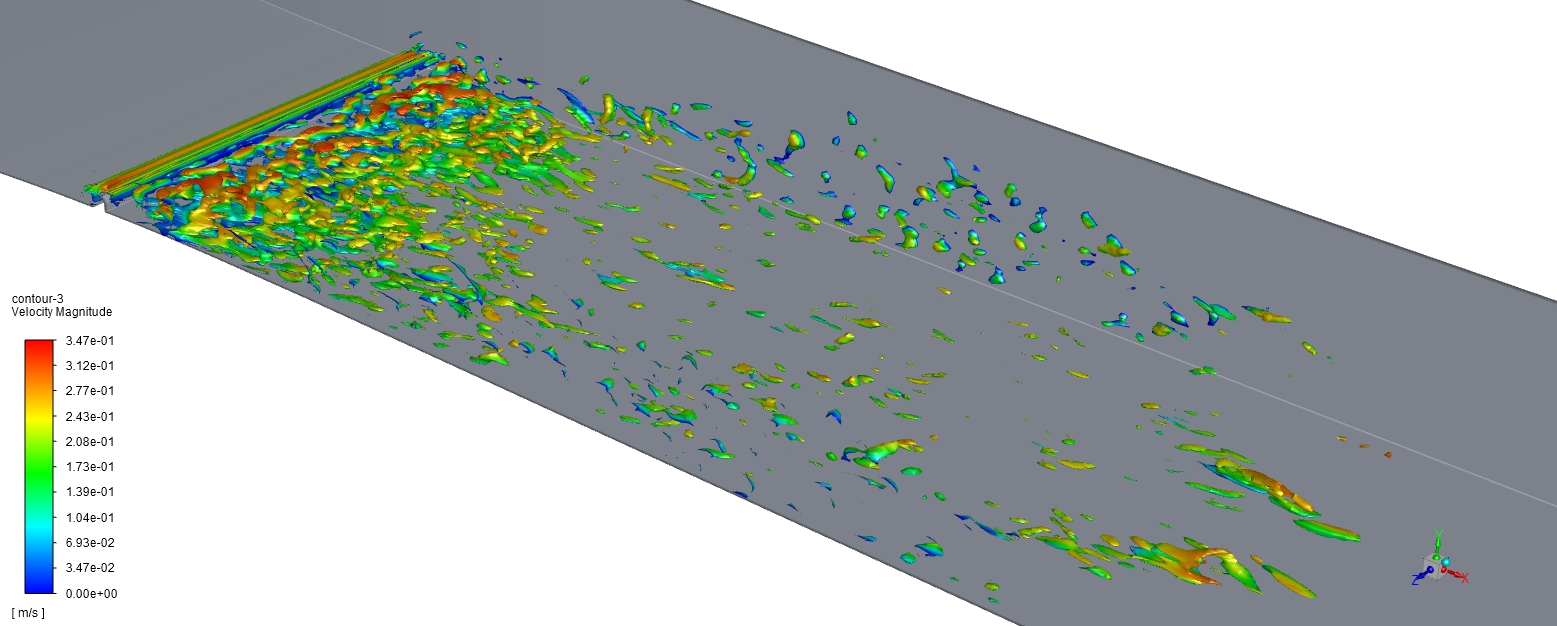
\includegraphics[width=1\linewidth]{../Assets/QM850-t16}
		\caption{Vortex structure at Q = -850 и t = 1.6 с}
		\label{fig:qm850-t16}
	\end{figure}
	\newpage
	
В данной работе изучены различные методы моделирования турбулентных течений, их преимущества и недостатки, а также оценена производительность. Помимо этого изучены способы построения сеточной модели и создана оптимальная схема по работе над ней.

Расчет проводился методом моделирования крупных вихрей(LES) и подсеточной моделью WALE с коэффициентом $C_w = 0.325$. Эта комбинация позволила достаточно точно рассчитать турбулентное состояние пограничного слоя. Кроме того использовалась оптимальная схема построения сеточной модели, что сократило время генерации в несколько часов.

В результате проведенного моделирования канала в Ansys Fluent было оценено влияние вихрегенераторов на пограничный слой. Их наличие изменило скоростные характеристика потока за препятствием. Благодаря размещению вихрегенератора поперек образовался турбулентный режим движения. Появившиеся вихревые структуры воздействовали на стенки канала.

До изменений в потоке коэффициент трения составлял 0.4. После установки вихрегенератора значительное изменение в коэффициенте трения оказалось в правой части канала($z = -31$ мм), он вырос в 4.5 раза. В левой($z = 31$ мм) -- увеличение в 3 раза. А по центру канала($z = 0$ мм) в 2.25 раза. Но уже после вихрегенератора значение коэффициента снижалось, стремясь к значениям до изменения в канале.

В последующих исследованиях возможно изучение с другими условиями движения потока, количеством и вариациями вихрегенераторов.
	\addcontentsline{toc}{section}{Conclusion}
	\newpage
	\bibliography{../bib/bibliography}
	\addcontentsline{toc}{section}{References}
	\newpage
	\addcontentsline{toc}{section}{Acknowledgments}
	\begin{center}
		\Large\textbf{Acknowledgments}
	\end{center}
	\newpage
	\begin{center}
		\Large\textbf{Revision record}
	\end{center}
\end{document}